%%%%%%%%%%%%%%%%%%%%%%%%%%%%%%%%%%%%%%%%%%%%%%%%%%%%%%%%%%%%%%%%%%%%%%
% amspaper.tex --  LaTeX-based template for submissions to American 
% Meteorological Society journals
%
% Template developed by Amy Hendrickson, 2013, TeXnology Inc., 
% amyh@texnology.com, http://www.texnology.com
% following earlier work by Brian Papa, American Meteorological Society
%
% Email questions to latex@ametsoc.org.
%
%%%%%%%%%%%%%%%%%%%%%%%%%%%%%%%%%%%%%%%%%%%%%%%%%%%%%%%%%%%%%%%%%%%%%
% PREAMBLE
%%%%%%%%%%%%%%%%%%%%%%%%%%%%%%%%%%%%%%%%%%%%%%%%%%%%%%%%%%%%%%%%%%%%%

%% Start with one of the following:
% DOUBLE-SPACED VERSION FOR SUBMISSION TO THE AMS
\documentclass{ametsoc}

% TWO-COLUMN JOURNAL PAGE LAYOUT---FOR AUTHOR USE ONLY
% \documentclass[twocol]{ametsoc}

%%%%%%%%%%%%%%%%%%%%%%%%%%%%%%%%
%%% To be entered only if twocol option is used

\journal{jamc}

\usepackage{color}

%  Please choose a journal abbreviation to use above from the following list:
% 
%   jamc     (Journal of Applied Meteorology and Climatology)
%   jtech     (Journal of Atmospheric and Oceanic Technology)
%   jhm      (Journal of Hydrometeorology)
%   jpo     (Journal of Physical Oceanography)
%   jas      (Journal of Atmospheric Sciences)	
%   jcli      (Journal of Climate)
%   mwr      (Monthly Weather Review)
%   wcas      (Weather, Climate, and Society)
%   waf       (Weather and Forecasting)
%   bams (Bulletin of the American Meteorological Society)
%   ei    (Earth Interactions)

%%%%%%%%%%%%%%%%%%%%%%%%%%%%%%%%
%Citations should be of the form ``author year''  not ``author, year''
\bibpunct{(}{)}{;}{a}{}{,}

%%%%%%%%%%%%%%%%%%%%%%%%%%%%%%%%

%%% To be entered by author:

%% May use \\ to break lines in title:

\title{High-resolution regional climate model evaluation using variable-resolution CESM over California}

%%% Enter authors' names, as you see in this example:
%%% Use \correspondingauthor{} and \thanks{Current Affiliation:...}
%%% immediately following the appropriate author.
%%%
%%% Note that the \correspondingauthor{} command is NECESSARY.
%%% The \thanks{} commands are OPTIONAL.

    \authors{Xingying Huang, \correspondingauthor{Xingying Huang, 
     Department of Land, Air and Water Resources,
     University of California Davis, Davis, CA 95616.}
  Alan M. Rhoades and Paul A. Ullrich}

     \affiliation{Department of Land, Air and Water Resources, University of Califonia, Davis}

\email{xyhuang@ucdavis.edu}


    \extraauthor{Colin M. Zarzycki}
    \extraaffil{National Center for Atmospheric Research}


%%%%%%%%%%%%%%%%%%%%%%%%%%%%%%%%%%%%%%%%%%%%%%%%%%%%%%%%%%%%%%%%%%%%%
% ABSTRACT
%
% Enter your Abstract here

\abstract{} 

\begin{document}


%% Necessary!
\maketitle


%%%%%%%%%%%%%%%%%%%%%%%%%%%%%%%%%%%%%%%%%%%%%%%%%%%%%%%%%%%%%%%%%%%%%
% MAIN BODY OF PAPER
%%%%%%%%%%%%%%%%%%%%%%%%%%%%%%%%%%%%%%%%%%%%%%%%%%%%%%%%%%%%%%%%%%%%%
%
\section{Introduction}

Global climate models (GCMs) have been widely used to simulate both past and future climate. Although GCMs have been demonstrated to successfully represent large-scale features of the climate system, they are usually employed at coarse resolutions ($\sim$1 degree), largely due to computational limitations. Global climate reanalysis datasets, which assimilate climate observations using a climate model, can represent a best estimate of historical weather patterns, but still have relatively low resolutions no finer than 0.5$^\circ$ {\color{red}[References]}. Consequently, regional climate is not well captured by either GCMs or global reanalysis datasets.  However, dynamical processes at unrepresented scales are significantly drivers for regional and local climate variability, especially over complex terrain \citep{soares2012wrf}. In order to capture these fine-scale dynamical features, high horizontal resolution is needed to allow a more accurate representation of fine scale forcing, processes and interactions (see, for example, \cite{leung2003regional, rauscher2010resolution}). We anticipate a better representation of regional climate information can better inform local stakeholders and policymakers towards action on climate change and mitigation.

In order to model regional climate at high spatial and temporal resolution over a limited area, downscaling methods have been developed. There are largely two approaches for downscaling:  The first is statistical downscaling, which aims to estimate fine scale behavior via analysis of the relationships between observed variables at different scales \citep{fowler2007linking}. This method is empirical and cannot be used if the observed relationships do not hold with a changing climate \citep{soares2012wrf}. The second approach is dynamical downscaling, which uses a numerical model to simulate higher spatial resolution conditions in greater detail. Dynamical downscaling is popular and commonly employed, using nested limited-area models (LAMs) to model regional scales  \citep{laprise2008challenging}.  In this context, LAMs are typically referred as regional climate models (RCMs) when applying to climate scales. RCMs are forced by output of GCMs or reanalysis data, and have been widely used, particularly to capture physically consistent regional and local circulations at the needed spatial and time scales \citep{christensen2007regional, bukovsky2009precipitation, caldwell2009evaluation, mearns2012north}. More recently, variable-resolution global climate models (VRGCMs) have been more widely employed for modeling regional climate.  This approach uses a global model that includes high-resolution over a specific region and lower resolution over the remainder of the globe \citep{staniforth1978variable, fox1997finite}. VRGCMs have been demonstrated to be effective for regional climate studies and applications, owing to the advantages of traditional GCMs in representing large-scale features, at a reduced computational cost compared to uniform GCMs \citep{fox2001variable, fox2006variable, rauscher2013exploring, zarzycki2014using, zarzycki2014multidecadal, zarzycki2015localizedgrid}. 

Compared with RCMs, a key advantage of VRGCMs is the use a single, unified modeling framework, rather than a separate GCM and RCM. Thus VRGCMs avoid potential inconsistency between the global and regional domains, and naturally support two-way interaction between these domains without the need for nudging \citep{warner1997tutorial, mcdonald2003transparent, laprise2008challenging, mesinger2013limited}. However, in order to obtain deeper insight into the performance of these two modeling approaches, it is necessary to compare them directly. For the purposes of this paper, we will focus on the recently developed variable-resolution Community Earth System Model (varres-CESM) as our VRGCM of interest. CESM is a state-of-the-art Earth modeling framework developed at NCAR, consisting of atmospheric, oceanic, land and sea ice components \citep{neale2010description}. Although CESM has been well-used for uniform resolution modeling, variable-resolution in the Community Atmosphere Model�s (CAM) Spectral Element (SE) dynamical core has only been recently developed and has never be investigated for long-term regional climate simulation \citep{taylor2010compatible, zarzycki2014using}.  Consequently, the goal of this paper is to evaluate the performance of varres-CESM against gridded observational data, reanalysis data and as compared to a dynamically downscaled modeling strategy.  Our variable-resolution simulations will focus on relatively high resolutions for climate assessment, namely 28km and 14km regional resolution, which are much more typical for dynamically downscaled studies.  For comparison with dynamical downscaling, the Weather Research and Forecasting (WRF) model will be used \citep{skamarock2005coauthors}. WRF has gained wide acceptance to study regional climate over the past decade, showing its adequate capability in representation of mean fine-scale climate properties \citep{lo2008assessment, leung2009atmospheric, soares2012wrf}.  We anticipate that this assessment will add value in modeling mean regional climatology and improve our understanding about the effects of multi-scale processes in regional climate regulation.

%together with the traditional method of RCMs for the first time to see whether VRGCMs can show similar or even better ability in regional climate modeling. And simulations will be conducted at higher resolution than most former studies.  In this study, WRF (Weather Research and Forecasting)  For the VRGCM approach, 

Simulations using both varres-CESM and WRF have been performed for 26 years of historical climate with a regional domain centered on the state of California (CA). With its complex topography, coastal influences, and wide latitudinal range, this makes CA an excellent test bed for high-resolution climate studies. Also, an understanding of local climate variability is incredibly important for policymakers and stakeholders in California due to its vast agricultural industry, wide demographics, and vulnerability to anthropogenically-induced climate change \citep{hayhoe2004emissions, cayan2008overview}. RCM simulations over California have also been conducted in previous studies \citep{leung2004mid, kanamitsu2007fifty, caldwell2009evaluation, pan2011influences, pierce2013probabilistic}. \cite{caldwell2009evaluation}, in particular, presented results from WRF (Weather Research and Forecasting) at 12km spatial resolution showing both the overall consistency and certain bias between simulations and observations \citep{caldwell2009evaluation}. The paper is organized as follows. Section 2 describes the model set up, evaluation methods and verification data. In Section 3, results are demonstrated focusing on 2 m temperature (Ts) and precipitation (Pr). Key results are summarized and further discussion is made in section 4.

\section{Models and Methodology}

\subsection{Simulation design} 

{\color{red}All simulations use the AMIP protocols with prescribed sea-surface temperatures.  The ocean model is disabled.} 

\subsubsection{WRF} 

The fully compressible non-hydrostatic WRF-ARW model, version 3.5.1 is used. ERA-Interim pressure-level reanalysis was used to provide initial, lateral conditions and sea surface temperatures (SST) for the domains every 6 hours. ERA-Interim reanalysis ($\sim$ 80 km) has been widely used and validated for its reliability as forcing data \citep{dee2011era}. Two simulations are conducted with a maximum horizontal resolution of 27km (WRF27) and 9km (WRF9) respectively, over the time period 1979-01-01 to 2005-12-31 (UTC).  The $\sim 10$ km resolutions are actually finer than most former studies for long-term climate.

The simulation domains are depicted in Figure \ref{fig:Figure1}, along with the grid-scale topographic height.  For the WRF27 simulation one domain is used.  For the WRF9 simulation, two nested domains are used with outer domain at 27km (same as the WRF27) and inner domain at 9km horizontal grid resolution, with two-way nesting enabled.  These choices have been made to satisfy the natural WRF aspect ratio of 3:1.  Both grids are centered on CA and have respectively, 120$\times$110 and 151$\times$172 grid points.  Around the boundaries 10 grid points are used as lateral relaxation zones.  Since simulations cover climatological time scales, SSTs are updated each 6 hours. In order to reduce the drift between forcing data and RCM, grid nudging \citep{stauffer1990use} was applied to the outer domain every 6 hours at all levels except the planetary boundary layer (PBL) as suggested by\cite{lo2008assessment}. This setup uses 41 vertical levels with top pressure at 50 hPa.

%(check if other settings should add here)

We use the following parameterization options for the standard settings: WSM 6-class graupel microphysics scheme \citep{hong2006wrf}, Kain-Fritsch cumulus scheme \citep{kain2004kain}, CAM shortwave and longwave radiation schemes \citep{collins2004description} {\color{red}(??)}. {\color{red} These settings are supported by the one-year test running result with different options.} Also, the Yonsei University (YSU) boundary layer scheme \citep{hong2006new}, and Noah Land Surface Model \citep{chen2001coupling} are chosen as commonly used (?? add citations here) for climate applications considering long-term reliability and computational cost.

\subsubsection{Varres-CESM}

CESM has been under development for nearly two decades, and has been used heavily in better understanding the effects of global climate change \citep{hurrell2013community}. Here, CAM version 5 (CAM5) and the Community Land Model (CLM) version 4 are used. As mentioned earlier, SE is currently the default dynamical core in CAM along with recently added variable-resolution grid support. For our study, the variable-resolution cubed-sphere grids are generated within both CAM and CLM with the open-source software package SQuadGen \citep{ullrich2014squadgen}.  The grids used are depicted in Figure \ref{fig:Figure2}.  These grids correspond to 0.25 degree ($\sim$ 28km) and 0.125 degree ($\sim$ 14km) maximum horizontal resolution, with 1 degree resolution away from the regional domain.  These resolutions have been selected since CAM-SE naturally supports a 2:1 aspect ratio, meaning there are two transition layers from 1 degree to 0.25 degree, and one additional transition from 0.25 degree to 0.125 degree.  As with the WRF simulations, the time period from 1979-01-01 to 2005-12-31 (UTC). {\color{red} Corresponding fine-scale topography files have been produced.} Land surface data at 50 km resolution is used. {\color{red} Tuning parameters are not modified from their default configuration.} Greenhouse gas (GHG) concentrations are prescribed based on historical observations. SSTs and ice coverage are supplied by the 1degree Hadley Centre Sea Ice and Sea Surface Temperature dataset (HadISST) \citep{hurrell2008new}. 

%Settings for Varres-CESM (adding). 
%Figure 2 shows the grid mesh for each simulation.

\subsubsection{Uniform resolution CESM?}

%{\color{red} These simulation use an earlier version of CAM, CAM5-FV.  Need to ask Michael for a write-up of this dataset.}

fvCAM5.1 
1979-2005 observed SST, sea ice, CO2 and other greenhouse gases
year 2000 climatology for the prescribed aerosols.

This dataset is described in additional detail in \cite{wehner2014resolution} and \cite{wehner2014effect}.  Note that the appendix of the latter paper lists parameters that are different from the public release.

\subsection{Datasets}

Our evaluation focuses on near surface air temperature and precipitation, representative of the mean regional climate and climate variability on monthly, season and annual time scales. Reanalysis and gridded observational datasets (described in Table \ref{tab:Table1}) are employed as reference.  These data products incorporate station measurements, satellite information and other observational data.  Although these products are generally based on similar measurements, they are scaled and gridded using different techniques, causing processing uncertainty except of measurement error. Variation between reference products represents observational uncertainty.  We acknowledge that reanalysis products are particularly sensitive to model choice and choice of assimilated observations and so cannot be treated as truth.  Our assessment focuses on the performance of the WRF and CESM simulations in terms of both mean behavior and variability.  

% Due to the uncertainties in observations, we use different sources of datasets including measurements from stations, high-resolution reanalysis data or satellite information. 

\paragraph{NARR:}  The North American Regional Reanalysis (NARR) \citep{mesinger2006north} provides dynamically downscaled data over North America at $\sim$ 32 km resolution and 3 hourly intervals from 1979 through present.  All major climatological variables are present in NARR, making it an excellent candidate for assessment of regional extremes.  Nonetheless, some inaccuracies have been identified in NARR that must be accounted for, including deficiencies in precipitation fields away from the continental US \citep{bukovsky2007brief}.

\paragraph{Daymet:}  Daymet is an extremely high resolution (1 km) gridded dataset with daily outputs covering the period of 1980 through 2013 and including total precipitation, humidity and minimum and maximum temperatures \citep{thornton1997generating, thornton1999improved, thornton2000simultaneous}.  The dataset is produced using an algorithmic technique that ingests point station measurements in conjunction with a truncated Gaussian weighting filter.  Some adjustments are made to account for topography.  Daymet is available through the Oak Ridge National Laboratory Distributed Active Archive Center (ORNL DAAC).

\paragraph{PRISM:}  The Parameter-elevation Regressions on Independent Slopes Model (PRISM) \citep{daly2008physiographically} supports a 4km gridded dataset obtained by taking point measurements and applying a weighted regression scheme that accounts for many factors affecting the local climatology.  The datasets include total precipitation and minimum, maximum and (derived) mean temperatures.  Monthly climatological variables are available for 1895 through 2014.  Daily data is available for the period 1981 through present, although the documentation is careful to state that since the observational input changes over time this data is not intended for multi-decadal trends.  This dataset will be used for detection and characterization of temperature and precipitation extremes.

\paragraph{UW:}  The UW daily gridded meteorological data is obtained from the Surface Water Modeling group at the University of Washington \citep{maurer2002long}.  UW Ts dataset is computed similarly to Pr, but without the topographic adjustment towards PRISM, and using a simple 6.1 K/km lapse rate.  {\color{red}More?}

{\color{red}NLDAS?}

%The UW daily gridded meteorological data is obtained from the Surface Water Modeling group at the University of Washington \citep{maurer2002long}. The PRISM monthly gridded climate observations is produced by the PRISM (Parameter elevation Regression on Independent Slopes Model) Climate Group, and the dataset is based on a larger network of station data and accounts for elevation and topographic effects (cite??). UW Ts dataset is computed similarly to Pr, but without the topographic adjustment towards PRISM, and using a simple 6.1 K/km lapse rate. The Daymet gridded daily meteorological observations also take into account areas of complex terrain. The National Oceanic and Atmospheric Administration (NOAA) Climate Prediction Center (CPC) dataset uses more stations than the UW data, but without topographic correction (cite??). The National Centers for Environmental Prediction (NCEP) North American Regional Reanalysis (NARR) is NCEP's high resolution combined model and assimilated dataset (cite??).

For sake of consistency, reference data are averaged to models' output resolution when showing the differences or calculating related statistical values (e.g. root mean square error (RMSE), bias, and correlation). Bilinear interpolation method is used for regular 2D grid. {\color{red}Bilinear interpolation is probably not the best technique; when the reference data is higher resolution than the model output you should average to a model grid cell. When the reference data is coarser resolution, it is usually not desirable to interpolate to a finer grid -- this does not take into account topographic features which can greatly affect the results.} Also, output from globally uniform CESM with 25km spatial resolution is compared together to see if variable-resolution CESM perform similarly or even better in modeling mean climatology \citep{bacmeister2014exploratory}. The first year was treated as model spin-up, thus, all the data analysis are based on the period from 1980 to 2005, i.e. 26 years.

%Since the future simulations by RCMs can only be forced by GCM output, here, ~1 degree output of CESM is also used to force WRF to explore the effects of different boundary and initial conditions comparing with ERA-Interim. 

In order to get in-depth analysis of California's varied climate regions, here we divide the state into 5 regional zones as Figure \ref{fig:} shows.

\subsection{Post-processing}

TempestRemap blah blah blah.

\section{Results}

The grid-scale topography for the different simulations are contrasted in Figure \ref{fig:Figure3}.  The higher resolution models provide a clearly improved representation of local topography.  This is important for understanding climate simulations since topography is an important driver for fine-scale dynamic processes, especially over complex terrain.  Some differences are also apparent between the 28km varres-CESM and 27km WRF model, particularly over the central valley, and indicative of different methodology for preparation of the topography dataset.  In this section, we assess the models' performance in terms of both temperature and precipitation.  In particular, our comparison will focus on daily maximum, minimum and average 2m temperatures (Tmax, Tmin and Tavg), and daily precipitation (Pr) both annually and seasonally. These variables are the most relevant for a base-line climate assessment.

\subsection{Computational Cost}

{\color{red} Short write-up here about the simulation time for uniform, varres and WRF}

\subsection{Temperature}

{\color{red}Are annual average Tmax, Tmin and Tavg actually good indicators?  It seems like it might be better to not mix seasons.  Maybe show JJA Tmin, JJA Tavg, JJA Tmax, DJF Tmin, DJF Tavg, and DJF Tmax instead?}

The annual average climatology of Tmax, Tmin and Tavg from varres-CESM, uniform CESM-FV, WRF and reference datasets over the simulation period are shown in Figures \ref{fig:Figure4}, \ref{fig:Figure5} and \ref{fig:Figure6}. Generally, simulations show similar regional patterns to observations, with a warmer central valley and southern deserts, colder northern coastal area and Sierra Nevadas mountain region. Both WRF and variable-resolution CESM demonstrate satisfactory {\color{red}(What is satisfactory?)} ability to model the annual climatology. Importantly, the higher resolution simulations perform better capturing fine features close to observations, especially for WRF 9km. 

The differences between model results and reference data are plotted in Figure \ref{fig:Figure7} for Tavg, highlighting some of the key differences between simulations, especially when considering individual climate zones.

Comparing with the uniform resolution CESM-FV simulation, varres-CESM performed similarly or even better in some cases, showing both improved modeling ability at high resolution.
 
However, these models do exhibit some differences when examining different climate zones. In particular, Tmax is larger in the central valley in both CESM and WRF, and WRF 9km shows much more obvious cold bias in other regions than other simulations. Varres-CESM perform better than WRF and uniform CESM, especially at higher resolution. However, Tmin is obviously warmer by both WRF and CESM, especially at coastal region and southern desert, resulting under-prediction of diurnal range. WRF and uniform CESM perform better than varres-CESM. Varres-CESM and WRF perform similarly, better than uniform CESM. Comparing with PRISM, models show overall underestimation, especially at coastal and mountain regions, however with relatively small bias at most region. The RMSE for these models are basically ranges from 1 to 3 K, as showed by Table 2. Overall, variable-resolution CESM 0.125 deg performs best for long-term annual results, however,WRF 9km has larger error than WRF 27km. (varres-CESM > WRF > uniform CESM). And  Correlations are high between simulations and observations ($>$0.95), especially for Tmax and Tavg. There are about $+$2 K SST bias near the coast between varres-CESM and WRF. This may explain part of the reason for the above results. NARR shows obvious differences from other gridded observations, however, uncertainty between observational datasets are much smaller than the models' biases, unlikely impacting our results.

%For annual Tmax: Overestimate for WRF 9km. RMSE: CESM0.125<CESM 0.25<WRF27<WRF9<CESM uniform 0.25 around 1 to 3
%For annual Tmin: WRF 27<WRF9<CESM uniform<CESM 0.125<CESM 0.25 RMSE: similar around 1-3; Obviously overestimate, 
%For annual Tavg: Ranked from best to worst, we observe variable-resolution CESM 0.125 $>$ WRF 9km $>$ WRF 27km $>$ variable-resolution CESM 0.25 $>$ uniform CESM.

The seasonal cycle of Tavg is showed in Figure \ref{fig:Figure8}. Models do show good consistency with reference data with about no larger than 2 K bias, mainly in coldest and hottest seasons. However, varres-CESM do show smaller bias than WRF at summer season except over mountain region, and WRF did better at winter season. Varres-CESM seems to be colder in winter and WRF is not hot enough in summer. And varres-CESM showed larger variability among seasons than observations, while WRF shows opposite trend. No obvious divergence can be detected between multi-scales, though coarser simulations even result a littler better than finer ones. Also, seasonal trends are similar among sub-zones, though showing diverse magnitudes, and models seem to perform less better over coastal region. As for the multi-year monthly variability, models are quite close to reference dataset around 4 K, except in winter season, especially at January, varres-CESM and WRF 9km show about half time and one time larger values respectively.

For CA, we are more interested in the summer season, especially the Tmax value for heat extreme analysis {\color{red} what heat extreme analysis?  isn't that a subject of future work?}. Here, the annually average summer Tmax from models and reference data are displayed in Figures \ref{fig:Figure9} and \ref{fig:Figure10}. CESM generally overestimates Tmax especially for uniform CESM except at coastal region, while WRF showed obviously negative bias expect at central valley. Varres-CESM with higher resolution performed best as proved by the statistics in Table \ref{tab:Table3}, however, WRF 27km show less error than WRF 9km. Overall, models especially varres-CESM 0.125d and WRF 9km still show fairly accuracy over most regions. The underlying reasons behind those differences can be manifold including the models' inner mechanism, the forcing data and the scale effects. In order to further investigate the models' ability for heat extreme detection, we also depicted the frequency distribution of Tmax constructed from 26 years summer daily data in Figure \ref{fig:Figure11} {\color{red} (Compute summary statistics -- mean, median, variance, skewness, kurtosis -- for each distribution and tabulate results)}. Normal {\color{red}?} distributions are showed by both models and observations, though biases are noticed between them (even within observations). {\color{red}[The gridded data show no instances of tempratures above 45$^\circ$ in the central valley.  Perhaps look back at weather station data to see if this is valid]} Models are more consistent with observations over upper bound than lower bound. For hot events detection, both varres-CESM and WRF 27km exhibit satisfactory performance over most regions. No obvious improvement is showed by higher resolution in varres-CESM.

{\color{red} Appearance of sea breeze in high resolution runs.  WRF cold bias over Nevada / Idaho in DJF Tavg.}

%WRF9 tends to be obviously colder than WRF27. No sure why???. And this results differ from Soares and Caldwell
%JJA Tmax: Variable resolution CESM with higher resolution performs better than at coarser resolution. RMSE 2 to 4; CESM 0.125<WRF9km<CESM 0.25<WRF27<CESM uniform; They have high correlations and the error is controlled between 1-2 Celsius. Overestimate for CESM, especially for uniform; underestimate for WRF;

\subsection{Precipitation}

The long-term annual average climatology of daily precipitation (Pr) from varres-CESM, WRF and reference dataset are displayed by Figures \ref{fig:Figure12} and \ref{fig:Figure13}. Comparing with observations, simulations do capture regional patterns of precipitation. Precipitation distributes mostly along the north coastal part and Sierra mountains, and relatively low over other regions. However, there exist obvious differences among simulations. Varres-CESM overestimate a little especially for coarser simulation at the western side of Sierras, and finer simulation has reduced that bias showing the improvementnt of orographic effects. Comparing with varres-CESM, uniform CESM shows little difference overall, though with obviously less bias over central valley. Notably, large difference showed between WRF 27km and WRF 9km. WRF 27km underestimated a little, but WRF 9 greatly showed obvious positive absolute error at North coastal part and the Sierra where maximum precipitation is distributed, and the relative bias can reach 50 percent. Overall, models perform satisfactorily except for WRF 9km, and varres-CESM 0.125d perform a little better than CESM 0.25d and WRF 27km, as further showed by the RMSE and bias value in Table \ref{tab:Table4}. Observations also demonstrate noticeable differences indicating uncertainty inherent in interpolating station data to a grid. However, these observations are still of the highest quality available and the uncertainty is relatively small comparing the simulations, and our conclusions can hold.

%annual Pr: WRF 9km can be high as 12mm (1.5 times); CESM 0.125<CESM 0.25 and WRF 27<WRF 9.
%PRISM and Daymet are similar, so did not show PRISM here.
%plot the relative error??
%the reasons behind the large bias of WRF 9???

%add some percentage descriptions???

The climatological annual cycle of precipitation averaged over each sub regions is presented in Figure \ref{fig:Figure14}. It can be seen that bias mainly occurred during rainy seasons especially in winter. WRF 27km is more consistent with observations than others. Varres-CESM is wetter especially in winter season. WRF 9km is too wetter. And WRF 27km is dryer. As temperature, varres-CESM showed larger variability among seasons than observations, while WRF 27km shows opposite trend. The seasonal trend proves what we know about the strong seasonality of California Pr with high values during the winter and almost no precipitation during the summer.  %add comments after the figure settled

In this way, we particularly showed the annually average winter precipitation from models and reference data as plotted in Figures \ref{fig:Figure15} and \ref{fig:Figure16}. We can see that models and reference data show similar pattern as annual, though the precipitations almost doubles in winter comparing with annual value. Varres-CESM still overestimate with larger absolute bias, especially at central valley, and higher resolution still performs better. Uniform CESM overestimate over part of northern coast and mountain regions. WRF 27km underestimate a little, and WRF 9km still greatly overestimate at North coastal region and the sierra region. Considering the relatively heavy winter precipitation, the relative error is still acceptable for Varres-CESM, uniform CESM and WRF 27km, with RMSE and bias values showed in Table \ref{tab:Table5}. Further, the frequency distribution of winter Pr constructed from 26 years daily data is depicted in Figure \ref{fig:Figure17}. It can be seen that varres-CESM is more consistent with observations except at Central Valley, where WRF 27km performs much better as former figures already showed. Varres-CESM 0.25d and varres-CESM 0.125d do not show meaningful differences. However, WRF 27km shows underprediction of rainy days, especially for moderately rainy events, and, not surprisingly, WRF 9km obviously over-prediction rainy days particular when raining goes stronger. For strong precipitation events, varres-CESM and WRF 27 shows satisfactory modeling ability over most regions except at Central Valley for varres-CESM, though observations also show uncertainties.

%This gives confidence for using varres-CESM in extreme precipitation studies. 

The positive bias of precipitation using WRF at high resolution has also been found in former studies. \cite{caldwell2009evaluation} gave a detailed discuss of the possible reasons, stating that bias comes from a variety of source like the model itself and partly the physics schemes. And this is out of the scope of this paper, further discussion can be found in former studies \citep{jankov2005impact, gallus2006comparison}.


%DJF Pr: WRF 9km can be high as 24mm (also 1.5 times). For RMSE value is around one for CESM 0.125<WRF 27<CESM 0.25 <WRF 9 (around 4) 

%Figure convective precipitation VS micro-physics scheme especially for WRF 9km

At last, a concise summary of model performance annually over CA is provided by the Taylor diagram (Figure \ref{fig:Figure18}). This diagram includes the spatial correlation between the simulated and observed fields, the RMS variability of simulations normalized by that in the observations, and mean biases from verification data symboled at (1,0). %check the plot and then add comments

%The angle between the x axis and the vector connecting the symbol and the origin indicates the spatial correlation between the simulated and ob- served fields. The distance from the origin indicates the RMS variability in the simulations normalized by that in the observations. Perfect agreement with verification data, with mean biases removed, would appear as a symbol plotted at (1, 0). Movement closer to (1, 0) between two simulations indicates improvement.

\section{Discussions and summary}

scale effect, extreme analysis, precipitation parameterization

%\section{Figures and tables}

% TABLES

\begin{table}
\caption{Reanalysis or statistically downscaled observational datasets} \label{tab:Table1}
\begin{center}
\begin{tabular}{lcccc}
\hline \textbf{Data source} & \textbf{Variables used} & \textbf{Spatial resolution} & \textbf{Temporal resolution} \\
\hline \textbf{UW} & Pr, T$_{min}$, T$_{max}$ & 0.125$^\circ$ & daily \\
\textbf{PRISM} & Pr, T$_{min}$, T$_{max}$, T$_{avg}$ & 4km & monthly/daily \\
\textbf{DAYMET} & Pr, T$_{min}$, T$_{max}$ & 1km & daily \\
\textbf{NCEP CPC} & Pr & 0.125$^\circ$ & daily \\
\textbf{NARR} & Pr, T$_{s}$ & 32km & daily \\
\hline
\end{tabular}
\end{center}
\end{table}

\begin{table}
\begin{center}
\caption{RMSE for annual temperature (California)} \label{tab:Table2}
\begin{tabular}{lcccc}
\hline \textbf{RMSE} & \textbf{UW}  & \textbf{PRISM} & \textbf{DAYMET} \\
\hline $    $ & T$_{max}$ $\     $  T$_{min}$ & T$_{max}$ $\     $  T$_{min}$ $\     $ T$_{avg}$& T$_{max}$ $\     $  T$_{min}$\\
\hline \textbf{Varres CESM 0.25d} & 1.605 $\     $ 3.035  & 2.098 $\     $ 2.393 $\     $ 1.753	&  2.109 $\     $ 3.170 \\
\textbf{Varres CESM 0.125d} & 1.226 $\     $ 2.804  & 1.772	$\     $ 2.227	$\     $1.501 &	1.871 $\     $	2.884\\
\textbf{Uniform CESM 0.25d} & 2.566 $\     $	2.558 &	2.949$\     $	2.437$\     $	2.418&	2.958$\     $	2.826 \\
\textbf{WRF 27km} & 1.710	 $\      $ 2.506	 $\     $ & 2.240	 $\     $1.729 $\     $	1.721 &	2.105	 $\     $2.691 \\
\textbf{WRF 9km} & 2.517	$\      $2.769&	2.732$\      $	1.764$\      $	1.420 & 2.581	$\      $ 2.752 \\
\hline
\end{tabular}
\end{center}
\end{table}

\begin{table}
\begin{center}
\caption{Bias for annual temperature (California)} \label{tab:Table3}
\begin{tabular}{lcccc}
\hline \textbf{BIAS} & \textbf{UW}  & \textbf{PRISM} & \textbf{DAYMET} \\
\hline $    $ & T$_{max}$ $\     $  T$_{min}$ & T$_{max}$ $\     $  T$_{min}$ $\     $ T$_{avg}$& T$_{max}$ $\     $  T$_{min}$\\
\hline \textbf{Varres CESM 0.25d} & -0.082$\     $	2.385 &	-0.353$\     $	1.296$\     $	-0.269 & 	-0.037 $\     $	2.256 \\
\textbf{Varres CESM 0.125d} & -0.241$\     $	2.229	& -0.559$\     $	1.130$\     $	-0.438 &	-0.224	$\     $ 2.031\\
\textbf{Uniform CESM 0.25d} & -0.409 $\     $	1.402	& -0.672	$\     $ 0.312	$\     $ -0.907	& -0.361$\     $	1.272 \\
\textbf{WRF 27km} & -0.379$\     $	1.409 &	-0.649$\     $	0.321$\     $	-0.729 &	-0.336$\     $	1.282 \\
\textbf{WRF 9km} & -1.805 $\     $	2.166 &	-2.123	$\     $ 1.067$\     $	-0.891	& -1.786$\     $	1.967 \\
\hline
\end{tabular}
\end{center}
\end{table}

\begin{table}
\begin{center}
\caption{RMSE and Bias for summer (JJA) maximum temperature (Tmax) (California)} \label{tab:Table4}
\begin{tabular}{lcccc}
\hline \textbf{Tmax} & \textbf{UW}  & \textbf{PRISM} & \textbf{DAYMET} \\
\hline $    $ & RMSE $\     $  Bias & RMSE $\     $  Bias & RMSE $\     $  Bias \\
\hline \textbf{Varres CESM 0.25d} & 2.324$\     $	0.982	& 2.932$\     $	0.631	& 2.810$\     $	1.177 \\
\textbf{Varres CESM 0.125d} &1.903	$\     $ 0.651	& 2.452	$\     $ 0.233 &	2.477 $\     $	0.824\\
\textbf{uniform CESM 0.25d} & 3.872$\     $	1.788	& 4.265		$\     $ 1.449 &	4.300	$\     $	1.988 \\
\textbf{WRF 27km} & 2.311$\     $	-0.574	& 2.924$\     $	-0.925 &	2.511	$\     $ -0.383 \\
\textbf{WRF 9km} & 3.319	$\     $ -2.274	& 3.470$\     $	-2.693 &	3.203	$\     $ -2.101\\
\hline
\end{tabular}
\end{center}
\end{table}

\begin{table}
\begin{center}
\caption{RMSE and Bias for annual Precipitation (all California)} \label{tab:Table5}
\begin{tabular}{lcccc}
\hline \textbf{Pr} & \textbf{CPC}  & \textbf{UW} & \textbf{PRISM} & \textbf{DAYMET} \\
\hline $    $ & RMSE $\     $  Bias & RMSE $\     $  Bias & RMSE $\     $  Bias & RMSE $\     $  Bias \\
\hline \textbf{Varres CESM 0.25d} & 0.590	$\     $ 0.370 &	0.604 $\     $	0.265 &	0.726	$\     $ 0.171 &	0.560$\     $	0.169 \\
\textbf{Varres CESM 0.125d} &0.481 $\     $ 	0.220 &	0.534 	$\     $ 	0.126 &	0.634 $\     $  0.050	& 0.510	$\     $  0.043\\
\textbf{uniform CESM 0.25d} & 0.551$\     $	0.118 &	0.601 $\     $	0.012 &	0.708$\     $	-0.082	& 0.603 $\     $	-0.083 \\
\textbf{WRF 27km} & 0.424$\     $	-0.210 &	0.586$\     $	-0.315 &	0.777$\     $	-0.409 &	0.650$\     $	-0.411 \\
\textbf{WRF 9km} & 2.204	 $\     $ 1.462 &	2.026$\     $	1.368	& 1.858 $\     $	1.292 &	1.986 $\     $	1.286\\
\hline
\end{tabular}
\end{center}
\end{table}

\begin{table}
\begin{center}
\caption{RMSE and Bias for DJF Pr} \label{tab:Table6}
\begin{tabular}{lcccc}
\hline \textbf{Pr} & \textbf{CPC}  & \textbf{UW} & \textbf{PRISM} & \textbf{DAYMET} \\
\hline $    $ & RMSE $\     $  Bias & RMSE $\     $  Bias & RMSE $\     $  Bias & RMSE $\     $  Bias \\
\hline \textbf{Varres CESM 0.25d} & 1.409	$\     $ 0.883	& 1.401	$\     $ 0.558	& 1.636 $\     $	0.465	& 1.310 $\     $	0.404 \\
\textbf{Varres CESM 0.125d} &1.236	$\     $ 0.666 &	1.273	$\     $  0.362 &	1.436 $\     $ 	0.307 &	1.210 $\     $ 	0.234\\
\textbf{uniform CESM 0.25d} & 1.353 $\     $	0.273	& 1.440$\     $	-0.052	& 1.566	$\     $ -0.146	& 1.419	$\     $ -0.206 \\
\textbf{WRF 27km} &0.918 $\     $	-0.396 &	1.331  $\     $	-0.721	& 1.588  $\     $	-0.815 &	1.389	 $\     $ -0.876 \\
\textbf{WRF 9km} & 4.244 $\     $2.562	& 3.801	$\     $ 2.257 &	3.538$\     $	2.203 &	3.782	$\     $ 2.132\\
\hline
\end{tabular}
\end{center}
\end{table}

%\subsection{Figures}

\begin{figure}
\begin{center}
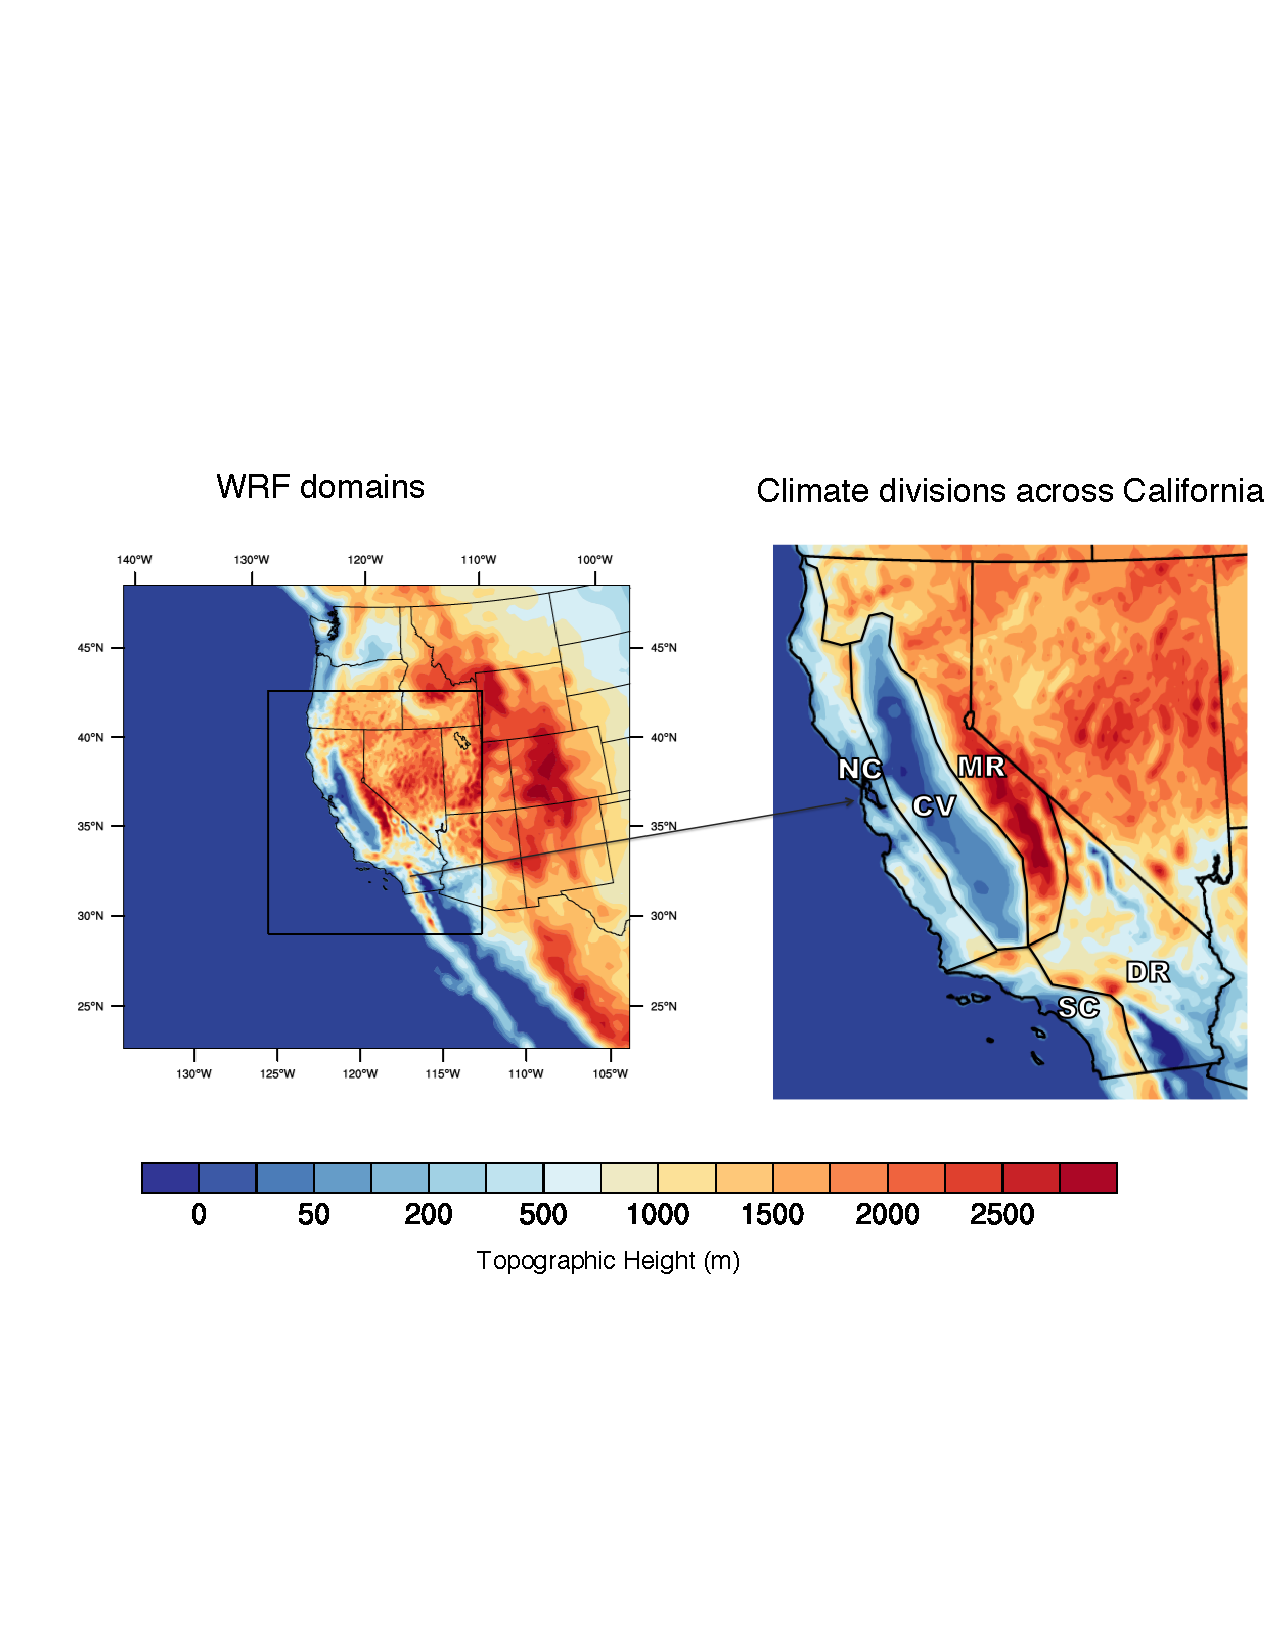
\includegraphics[width=6in]{wrf_domains.pdf}
\end{center}
\caption{Domains of WRF simulations (left: 9km, right: 27km) and topography height (meters). {\color{red}Use a single color bar for both plots. Try to match style of Figure 3. }} \label{fig:Figure1}
\end{figure}

\begin{figure}
\begin{center}
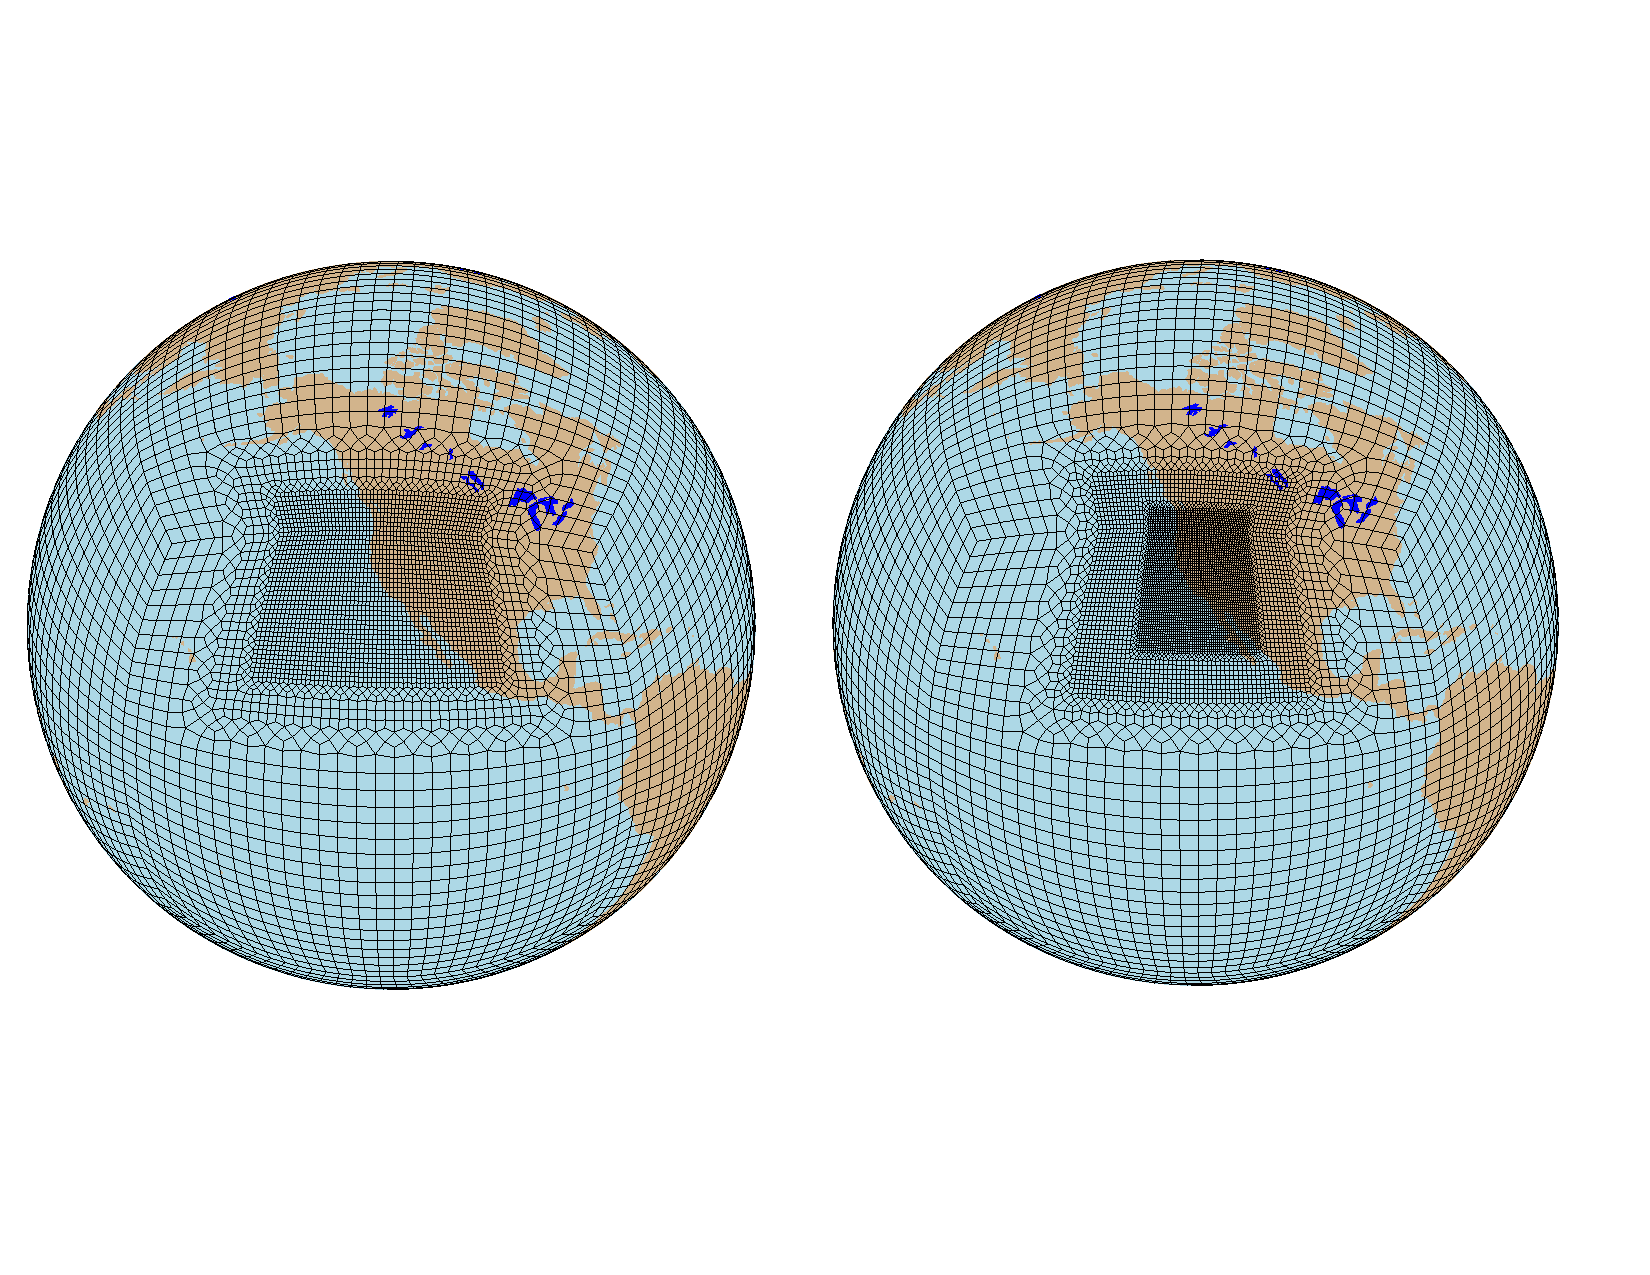
\includegraphics[width=6in]{varres-cesm_gridmesh.pdf}
\end{center}
\caption{The regionally refined mesh used for our varres-CESM simulations (Left: 0.25 degree, Right: 0.125 degree) {\color{red} The grid lines are too thick, making this image hard to see.  May need to re-render.}} \label{fig:Figure2}
\end{figure}

\begin{figure}
\begin{center}
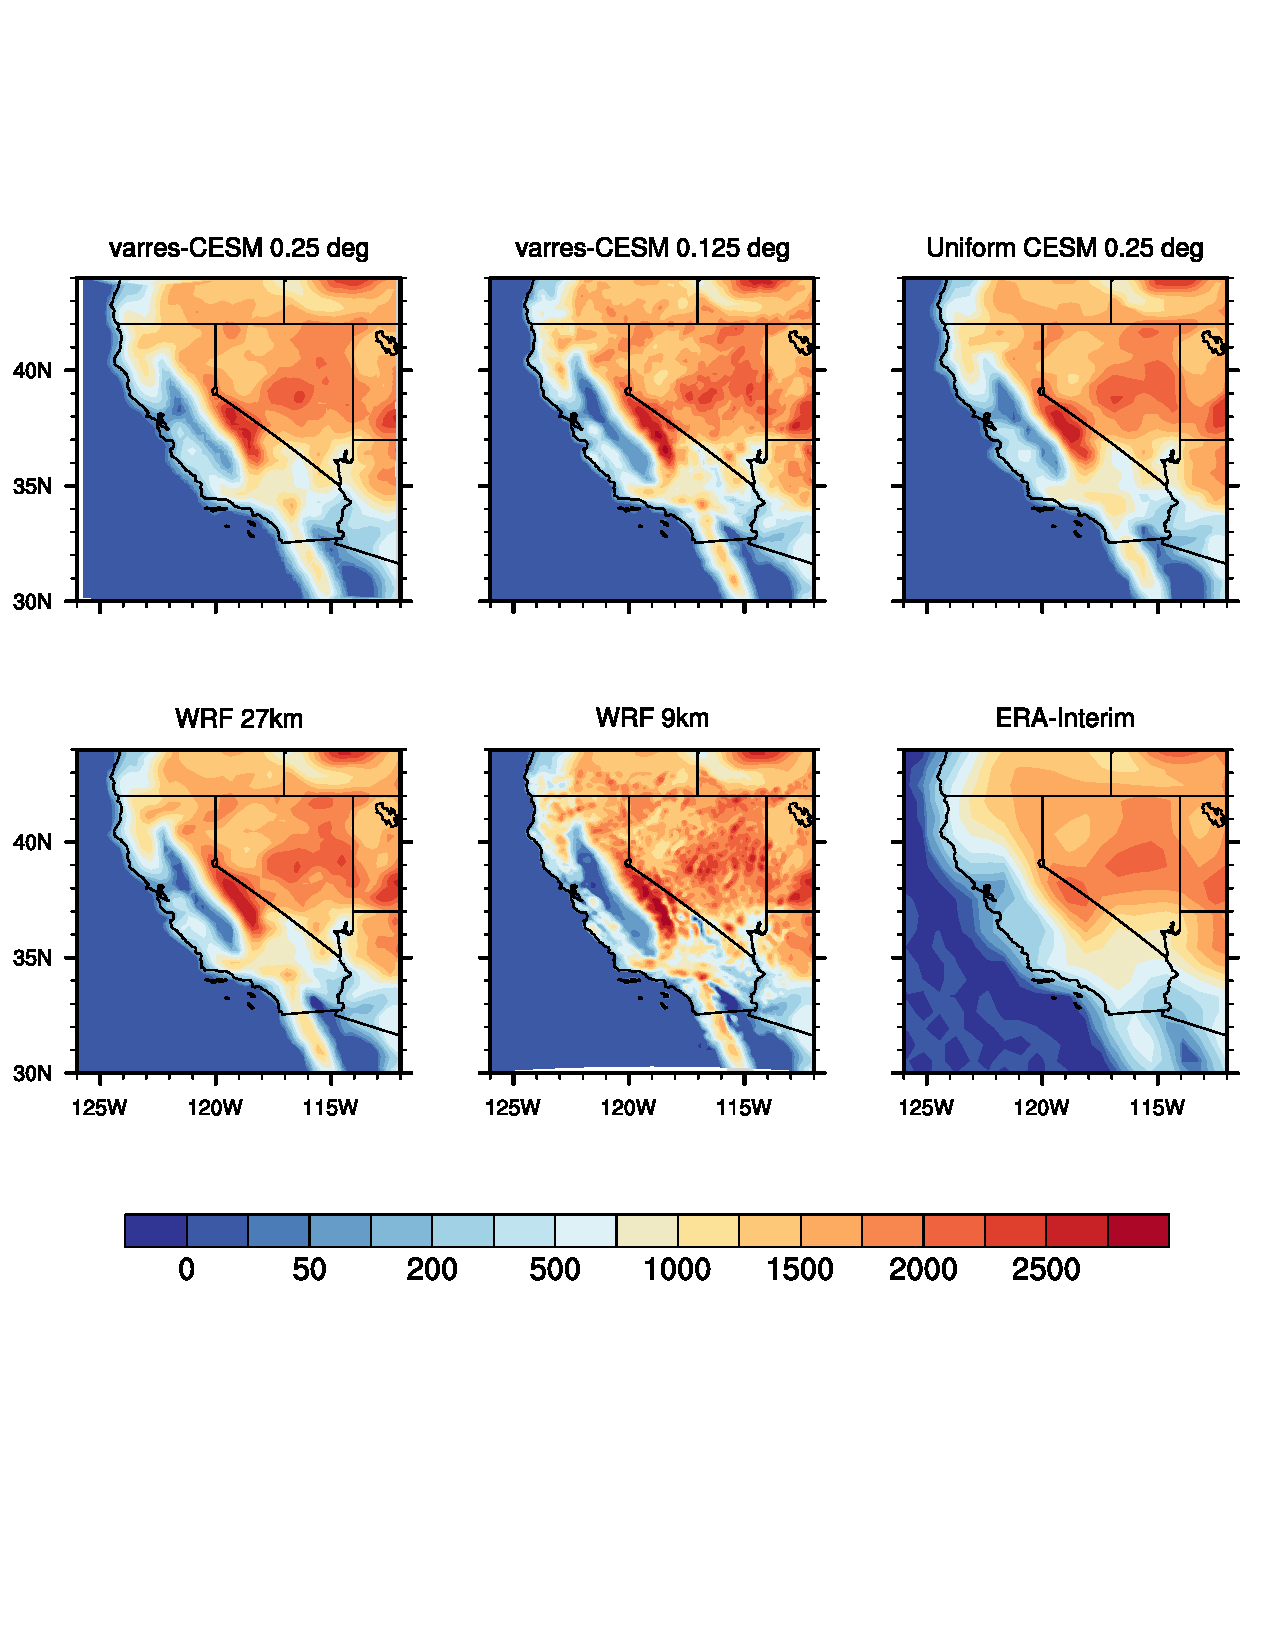
\includegraphics[width=6in]{topo.pdf}
\end{center}
\caption{Topography fields in meters (m) for (top left to bottom right) varres-CESM 28km, varres-CESM 14km, uniform CESM 25km, WRF 27km, WRF 9km and ERA-Interim. {\color{red}Use only a single color bar for all plots.  Match color scheme of Figure1.  Change 25km to 0.25$^\circ$ and 12.5km to 0.125$^\circ$.  Need to add a figure showing our 5 climate zones.}} \label{fig:Figure3}
\end{figure}

\begin{figure}
\begin{center}
\includegraphics[width=6in]{t2max.pdf}
\end{center}
\caption{Annual average daily maximum 2m temperatures (Tmax) from models and reference datasets (unit: $^\circ C$) {\color{red}Use only a single color bar for all plots.  Font size is also too small -- change to three rows -- first row CESM varres, second row CESM uniform + WRF, third row reference} } \label{fig:Figure4}
\end{figure}

\begin{figure}
\begin{center}
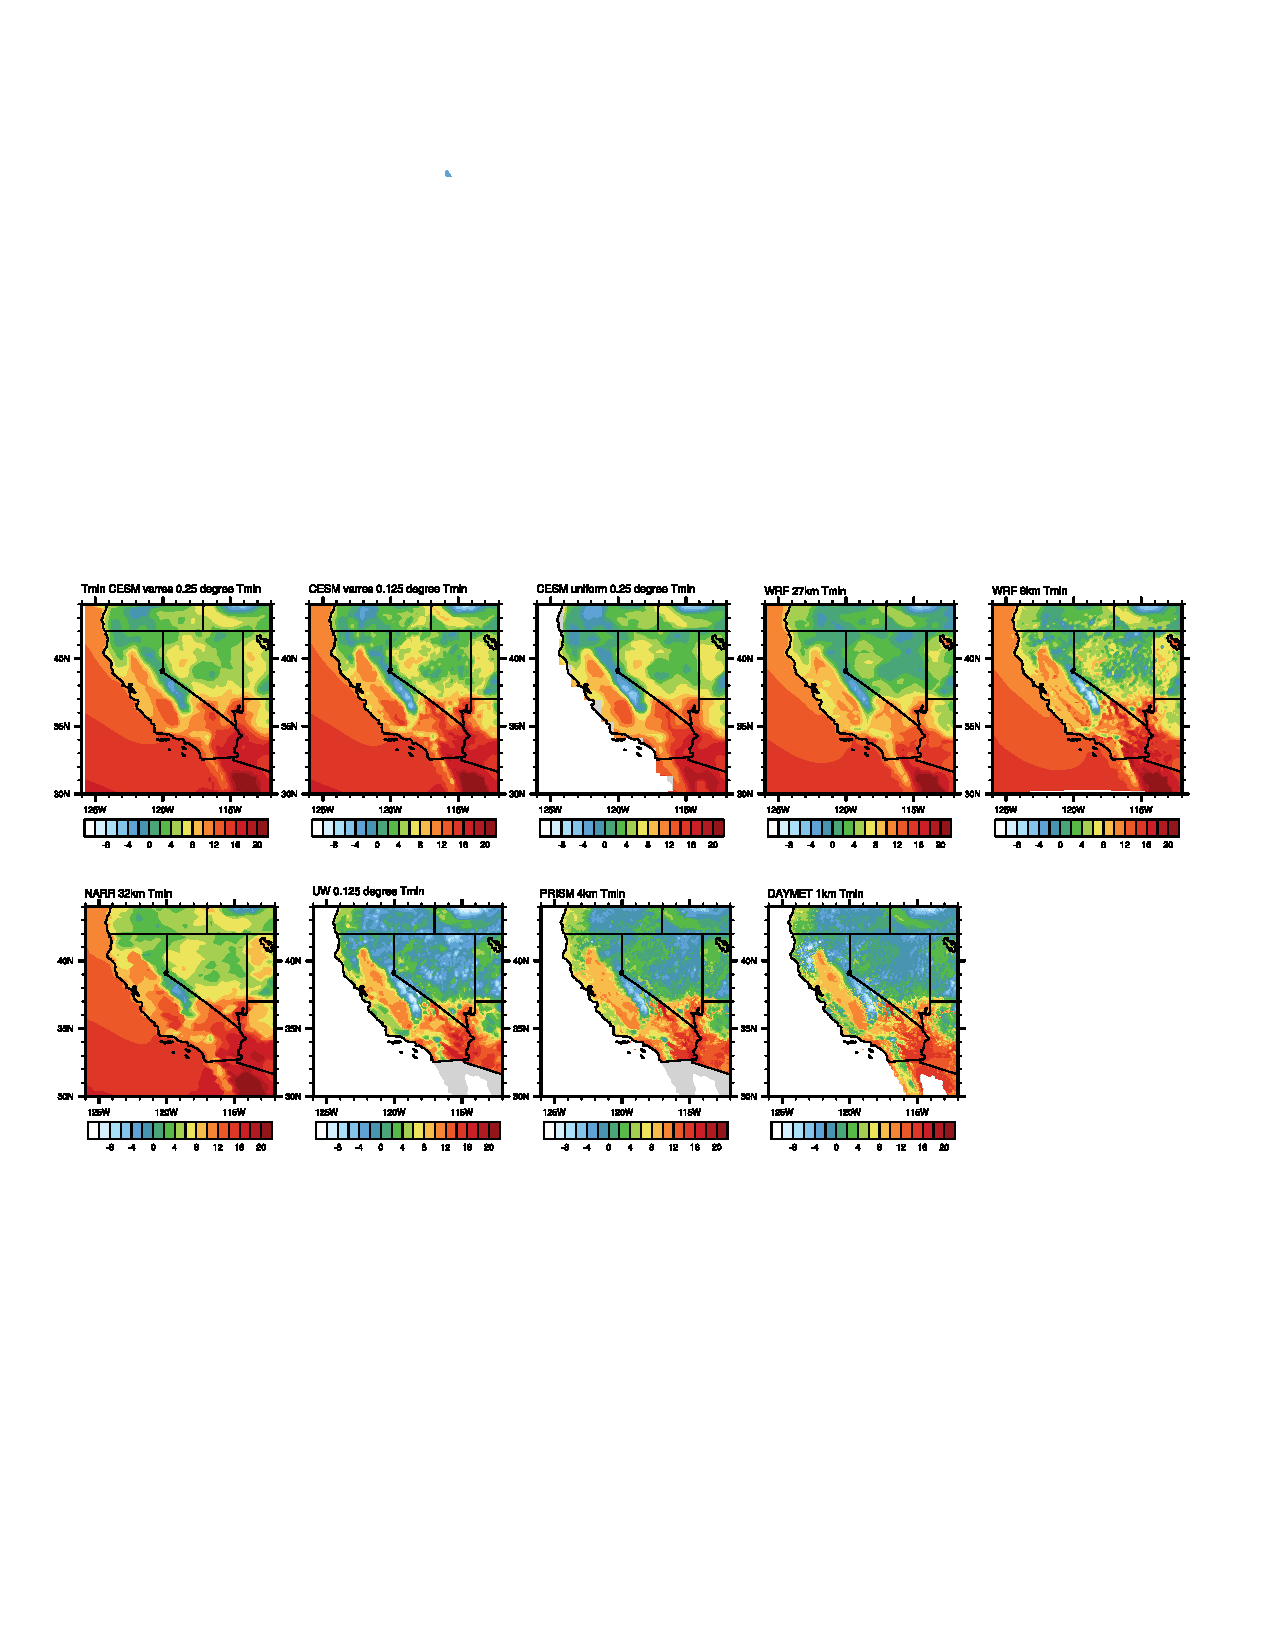
\includegraphics[width=6in]{t2min.pdf}
\end{center}
\caption{As Figure 4, but for daily minimum 2m temperatures (Tmin) {\color{red}Again switch to three rows, use only one label bar.}} \label{fig:Figure5}
\end{figure}

\begin{figure}
\begin{center}
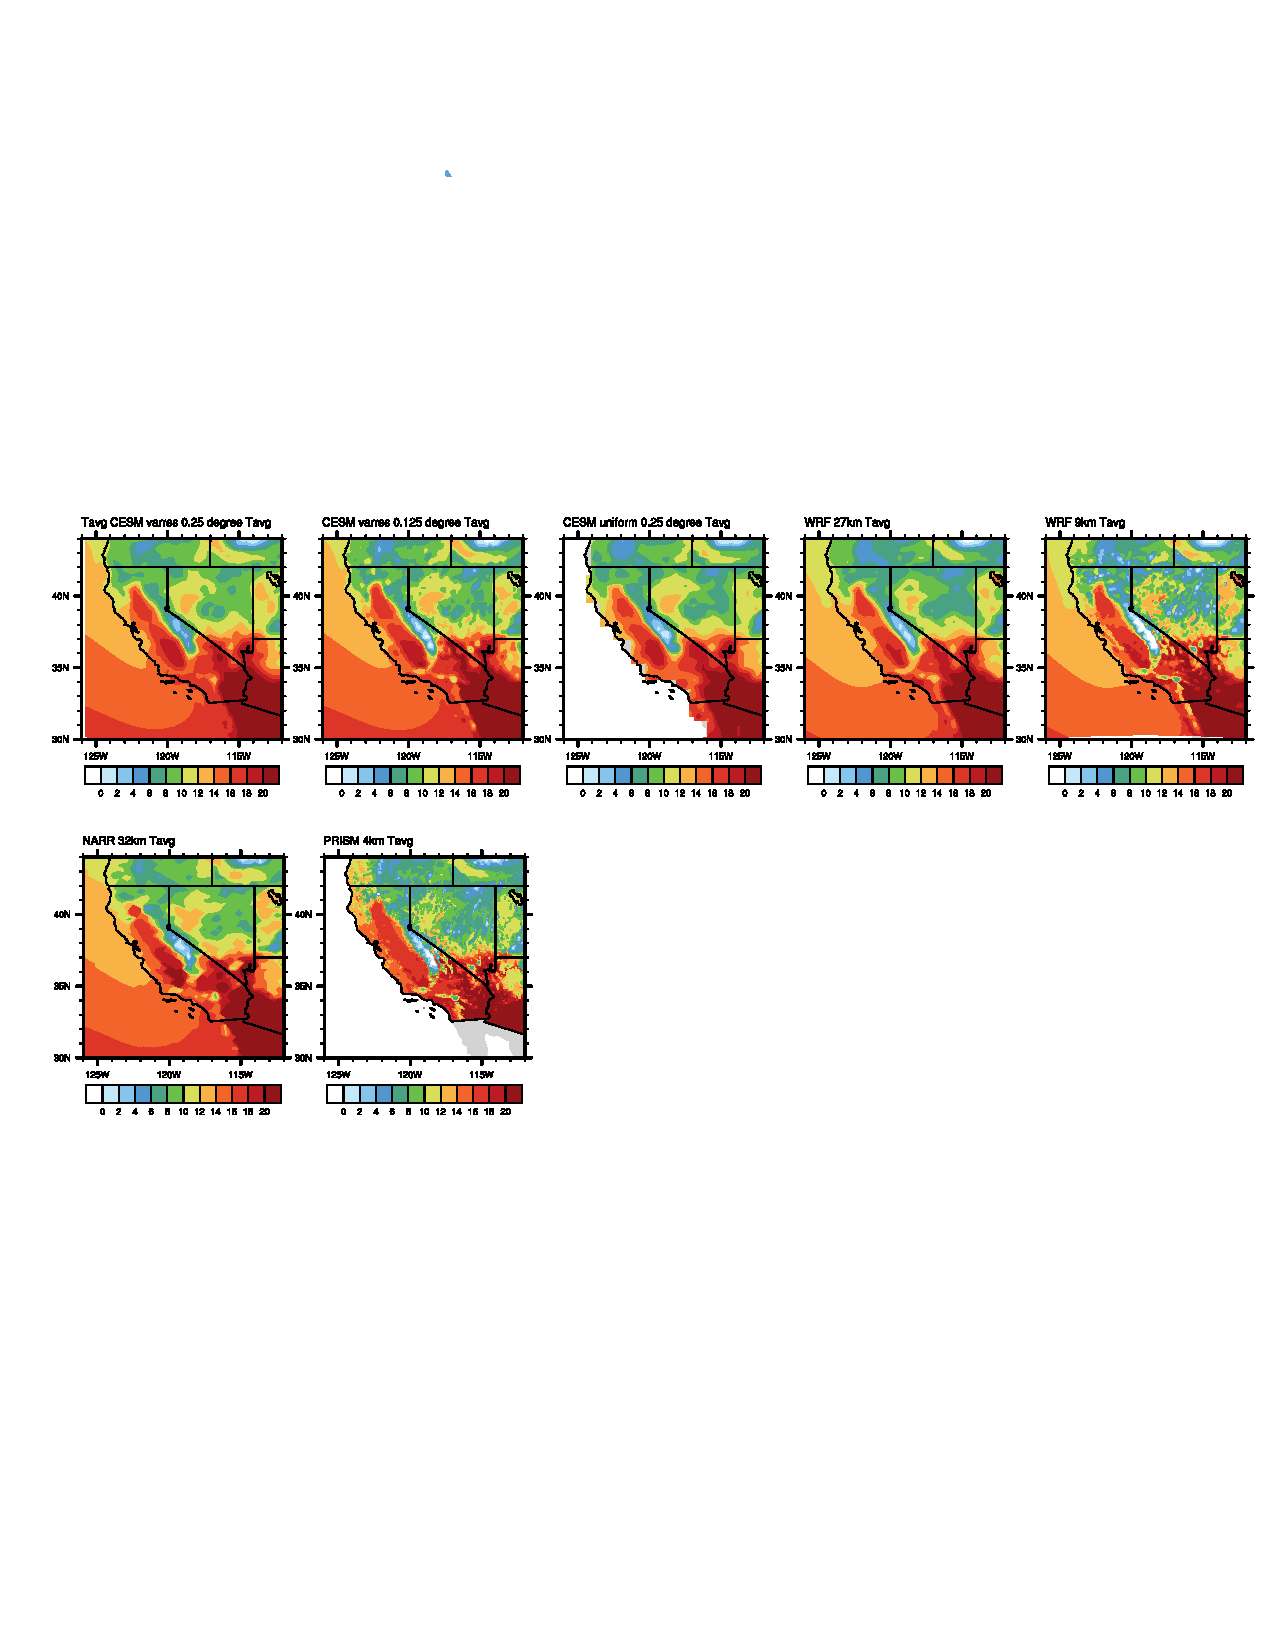
\includegraphics[width=6in]{t2avg.pdf}
\end{center}
\caption{As Figure 4, but for daily mean 2m temperatures (Tavg). {\color{red}Again switch to three rows, use only one label bar.}} \label{fig:Figure6}
\end{figure}

\begin{figure}
\begin{center}
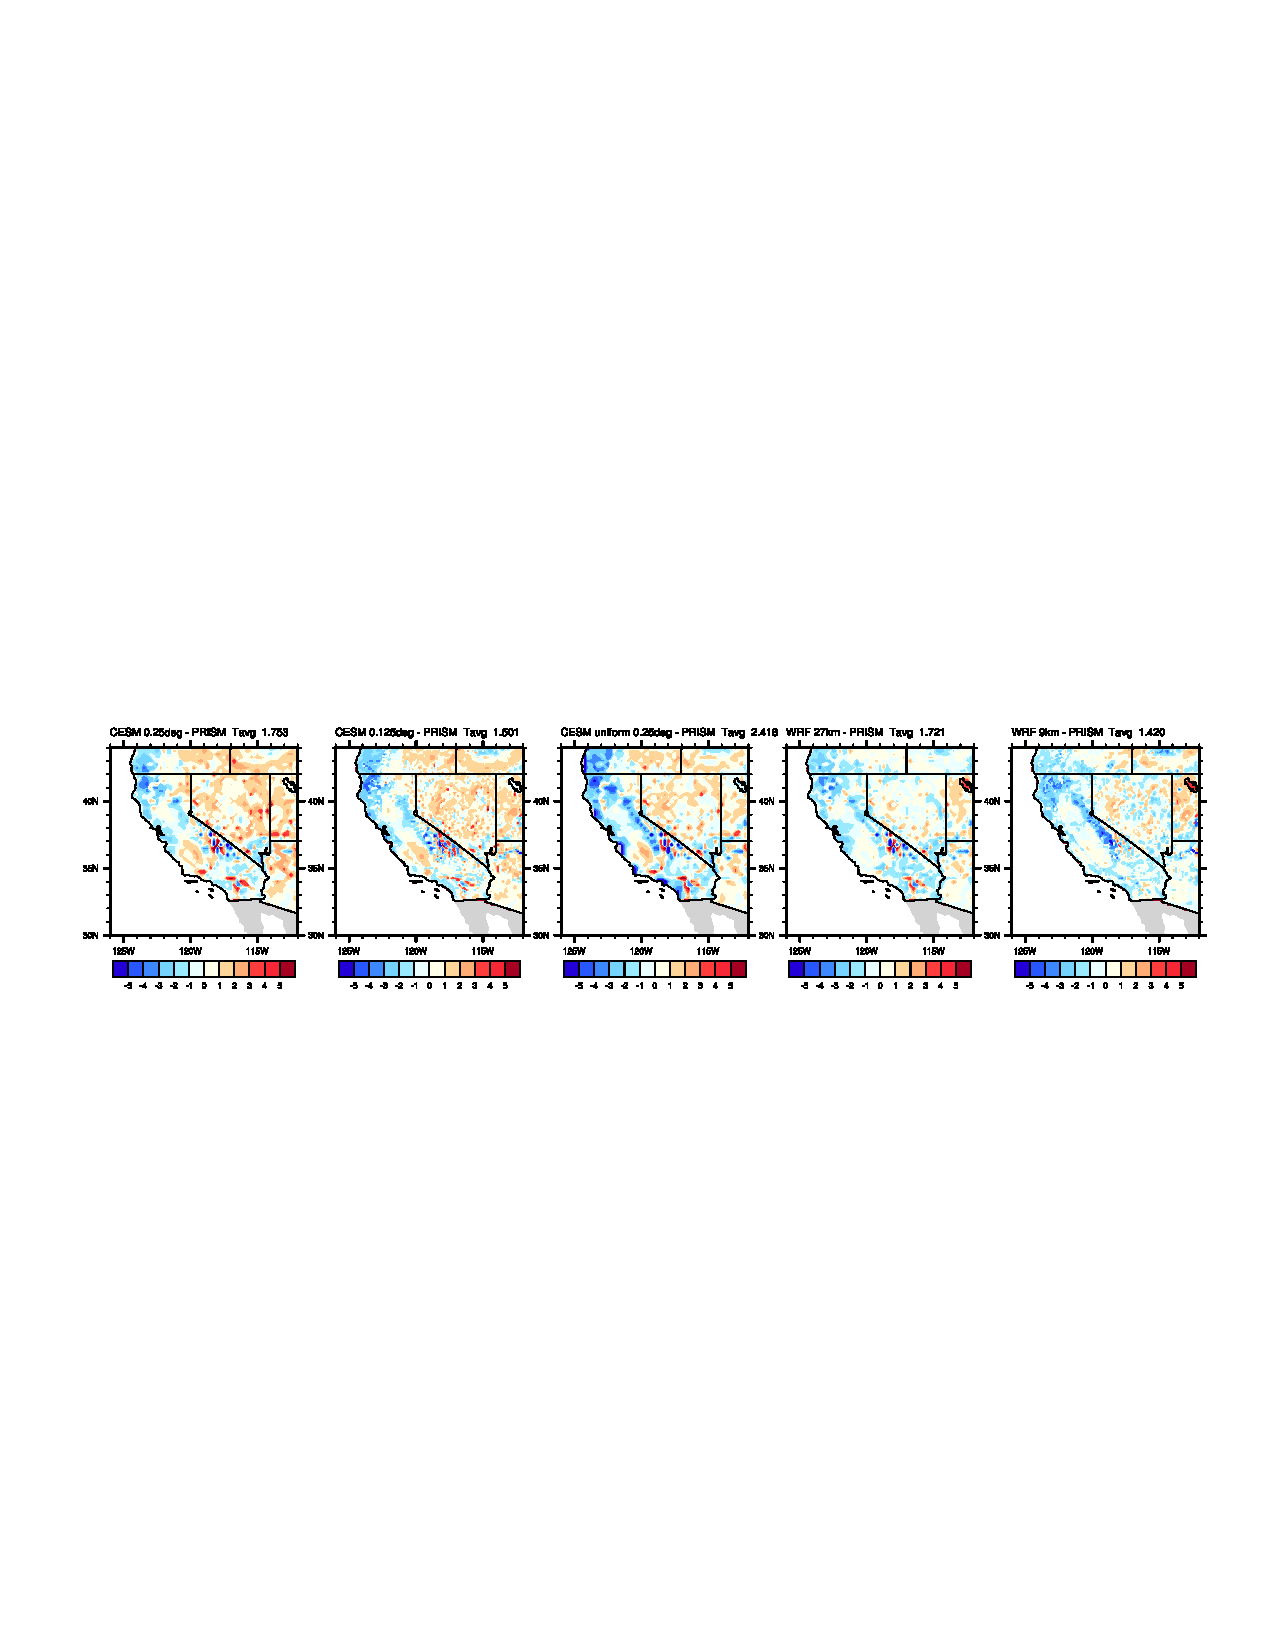
\includegraphics[width=6in]{t2avg_dif.pdf}
\end{center}
\caption{Difference between simulations and PRISM reference data for daily Tavg ($^\circ C$). {\color{red}Switch to two rows}} \label{fig:Figure7}
\end{figure}

\begin{figure}
\begin{center}
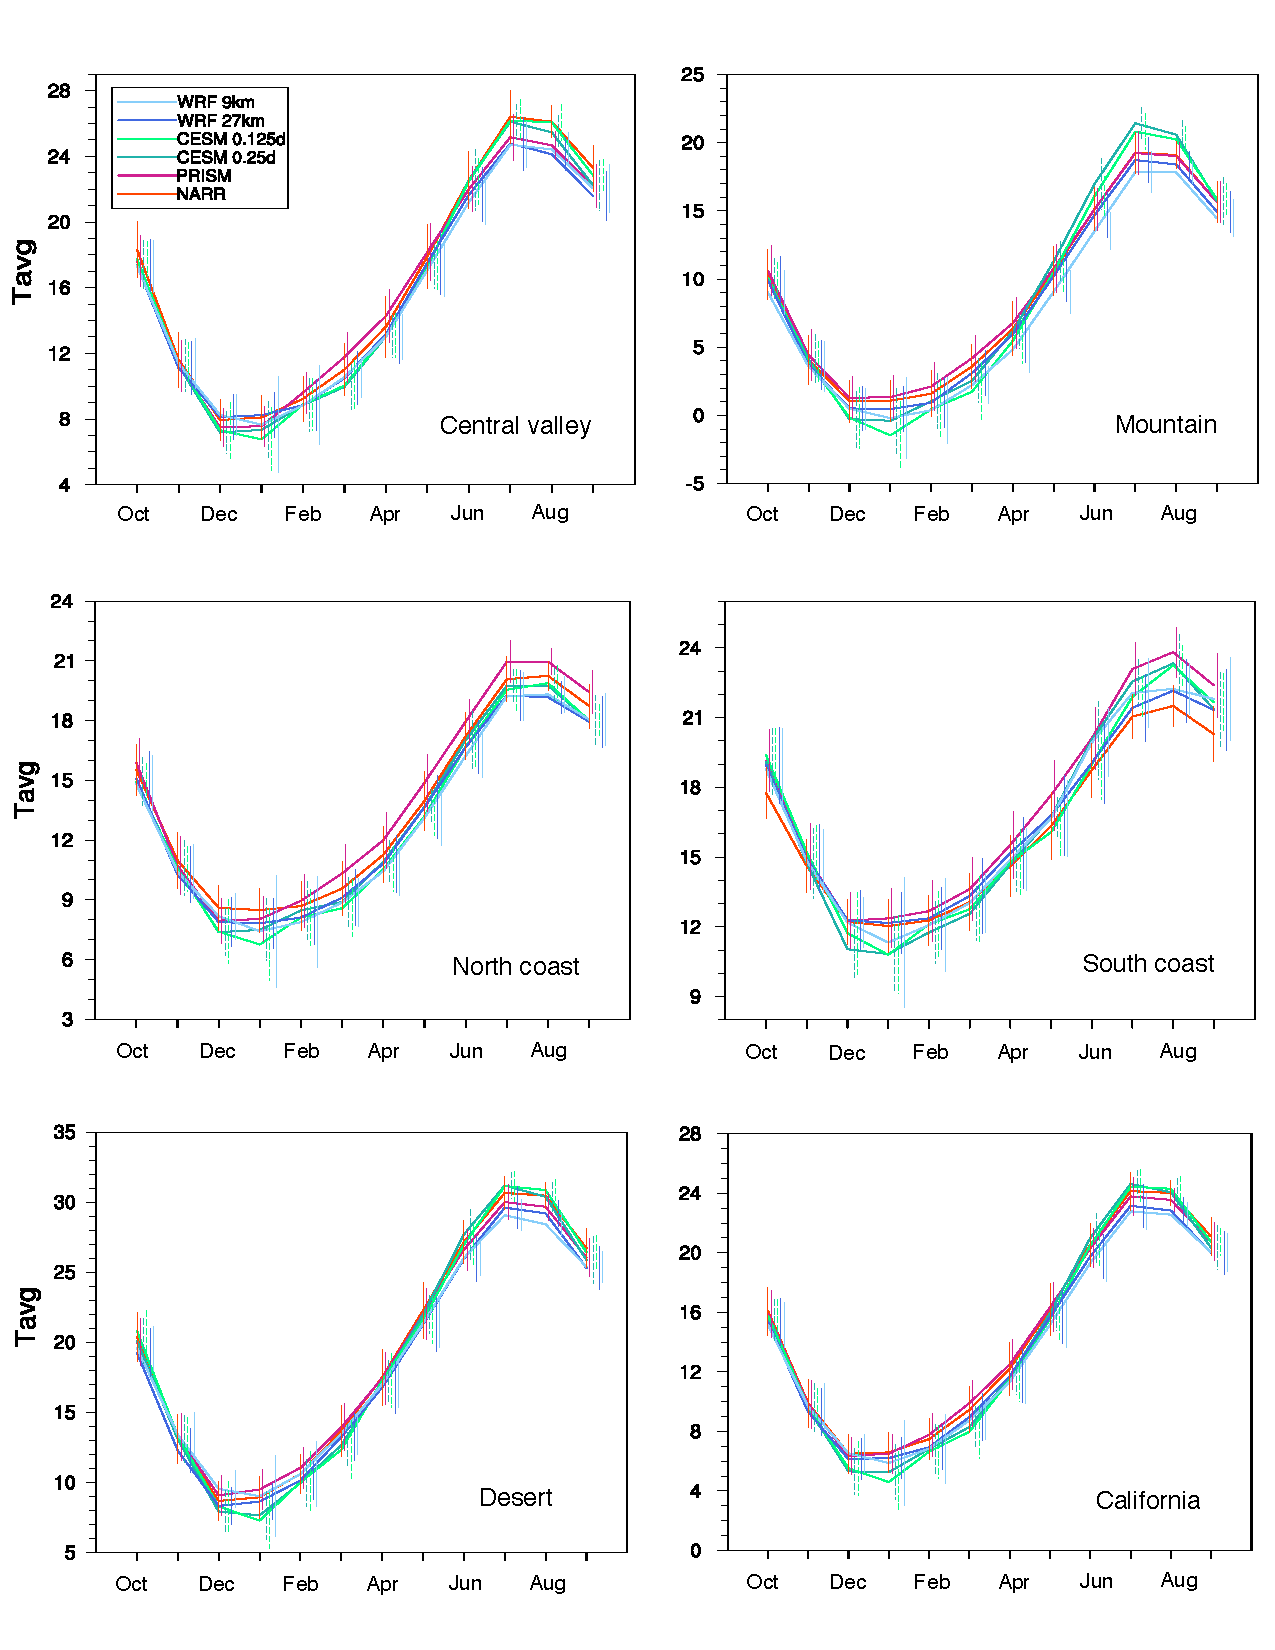
\includegraphics[width=6in]{trd_t2_allzones.pdf}
\end{center}
\caption{Seasonal cycle of monthly-average Tavg for each subzone ($^\circ C$) Errorbars represent ? values. {\color{red} Remove word ``month'' from plots. Change major tickmarks to be at each month.  ? is standard deviation?  Change to be January through December}} \label{fig:Figure8}
\end{figure}

\begin{figure}
\begin{center}
\includegraphics[width=6in]{t2max_JJA.pdf}
\end{center}
\caption{As Figure 4, but for summer Tmax. {\color{red}Use a single label bar.  Switch to three rows.  Is it possible to use the CAM data for CESM uniform 0.25 degrees so the ocean is shown?}} \label{fig:Figure9}
\end{figure}

\begin{figure}
\begin{center}
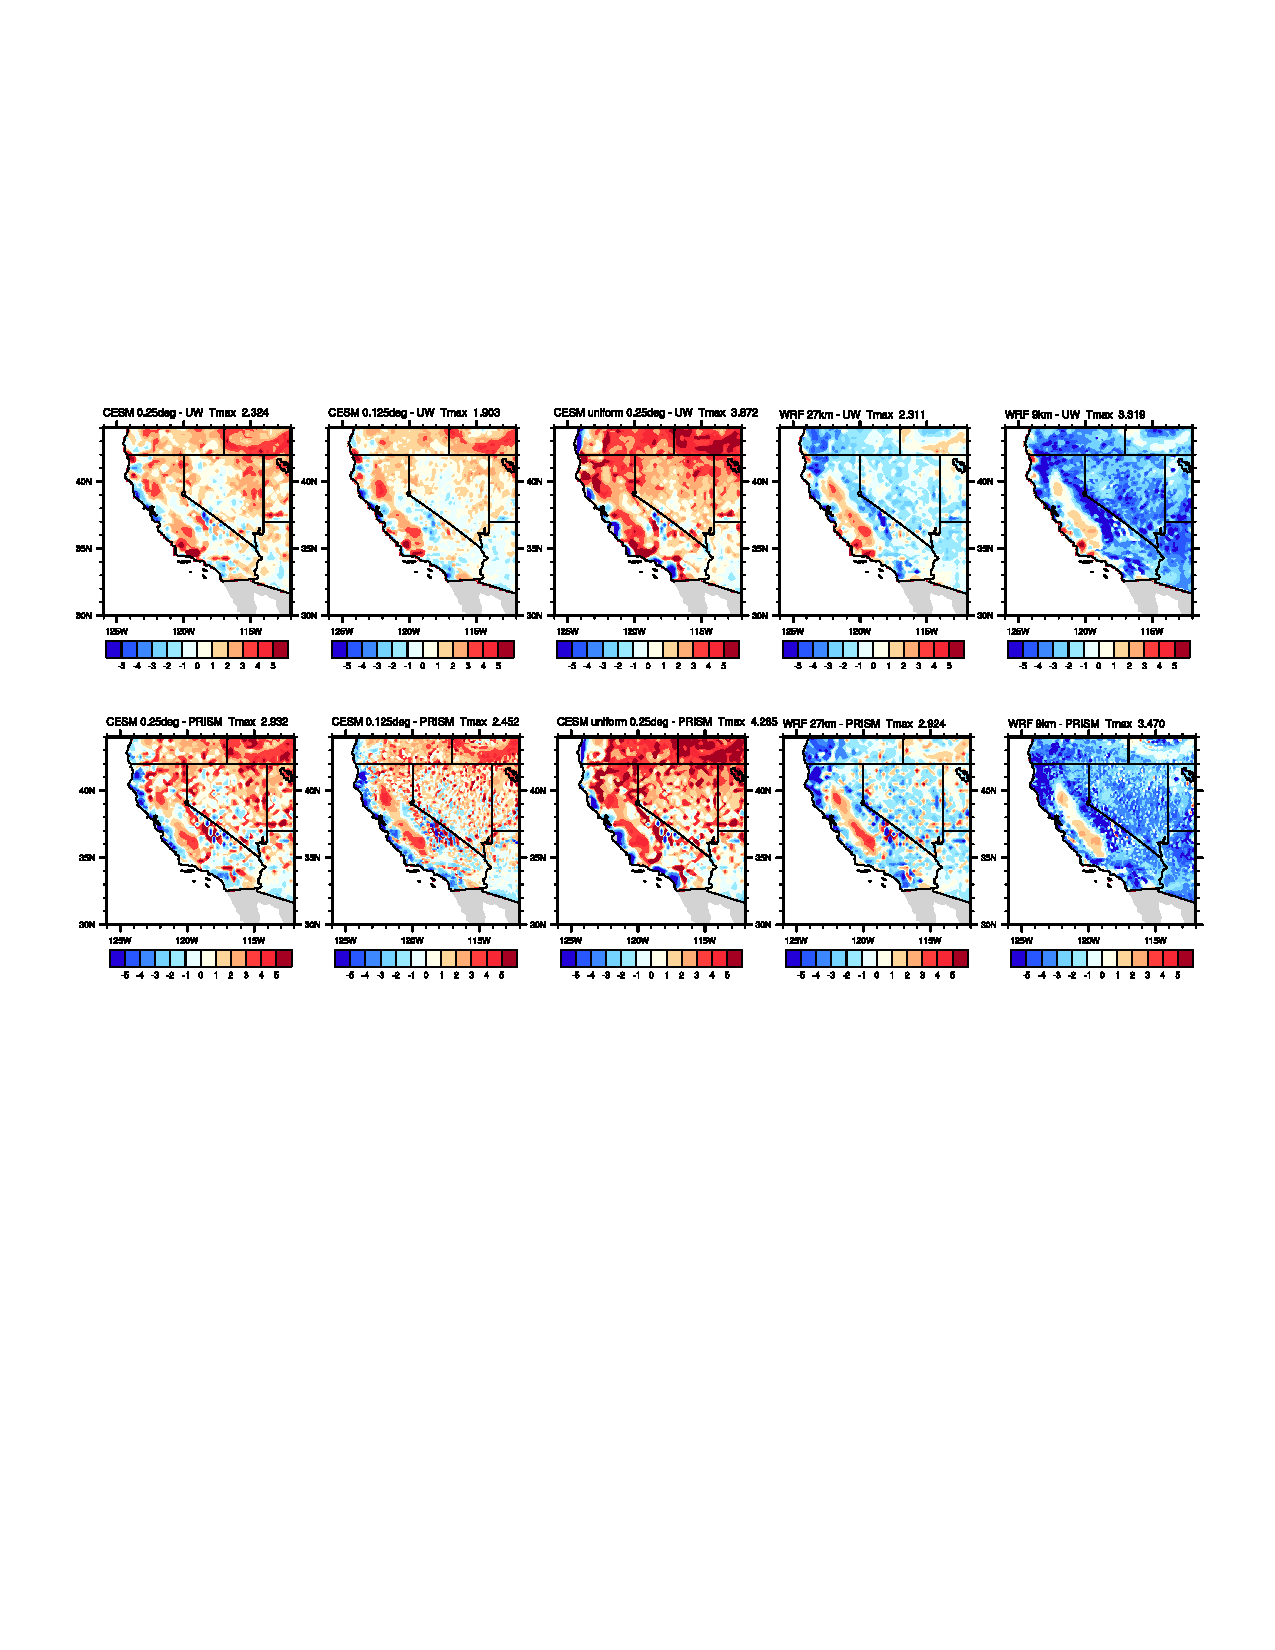
\includegraphics[width=6in]{t2max_JJA_dif.pdf}
\end{center}
\caption{As Figure 7 but for summer Tmax RMSE ($^\circ C$). {\color{red}Use a single label bar.  Switch to four rows.}} \label{fig:Figure10}
\end{figure}

\begin{figure}
\begin{center}
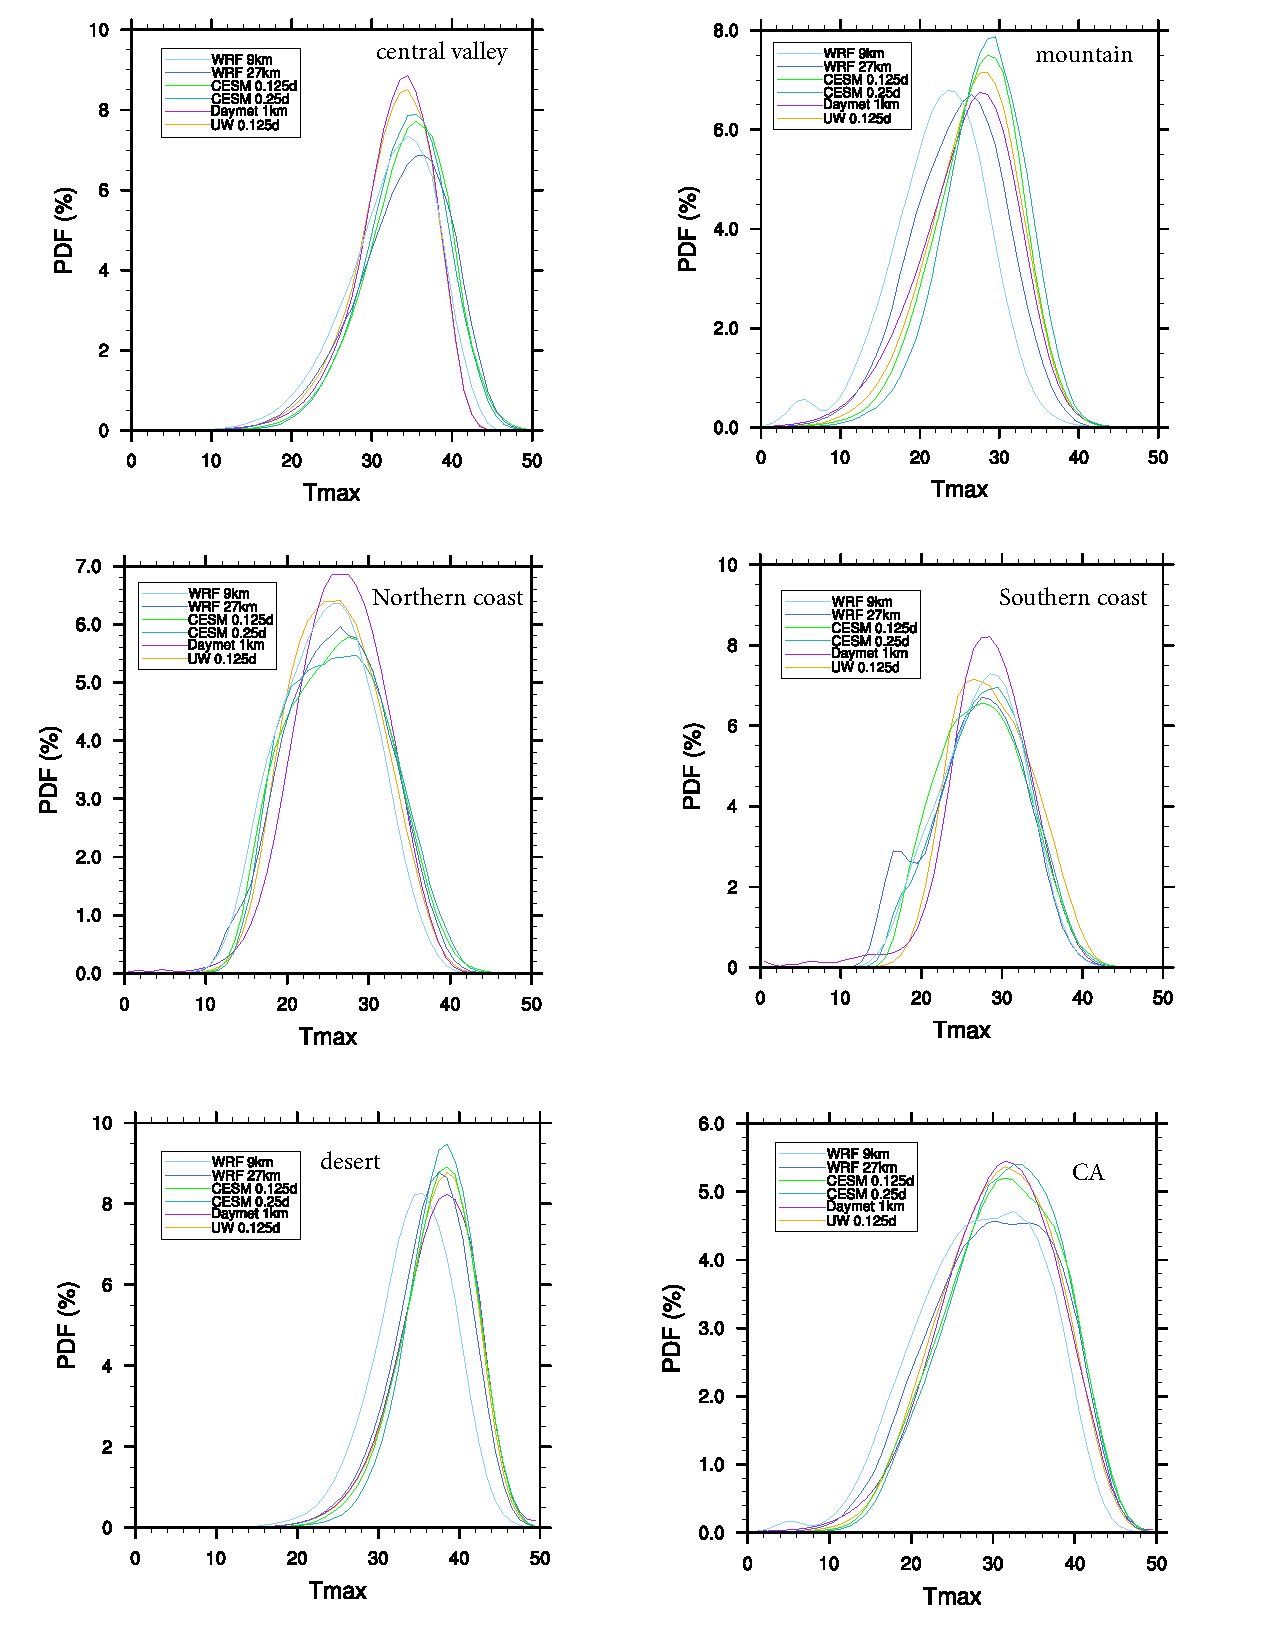
\includegraphics[width=6in]{PDF_t2max_allzones_JJA.pdf}
\end{center}
\caption{Frequency distribution of summer Tmax ($^\circ C$). {\color{red}Change vertical range to [0,10] in all plots.  Change ``central valley'' to ``Central valley'', ``mountain'' to ``Mountain'', ``desert'' to ``Desert'' and ``CA'' to ``California.''  Use only one legend.  Remove ``Tmax'' from horizontal label in all plots.  Change vertical label to ``Frequency (\%)''.}} \label{fig:Figure11}
\end{figure}

\begin{figure}
\begin{center}
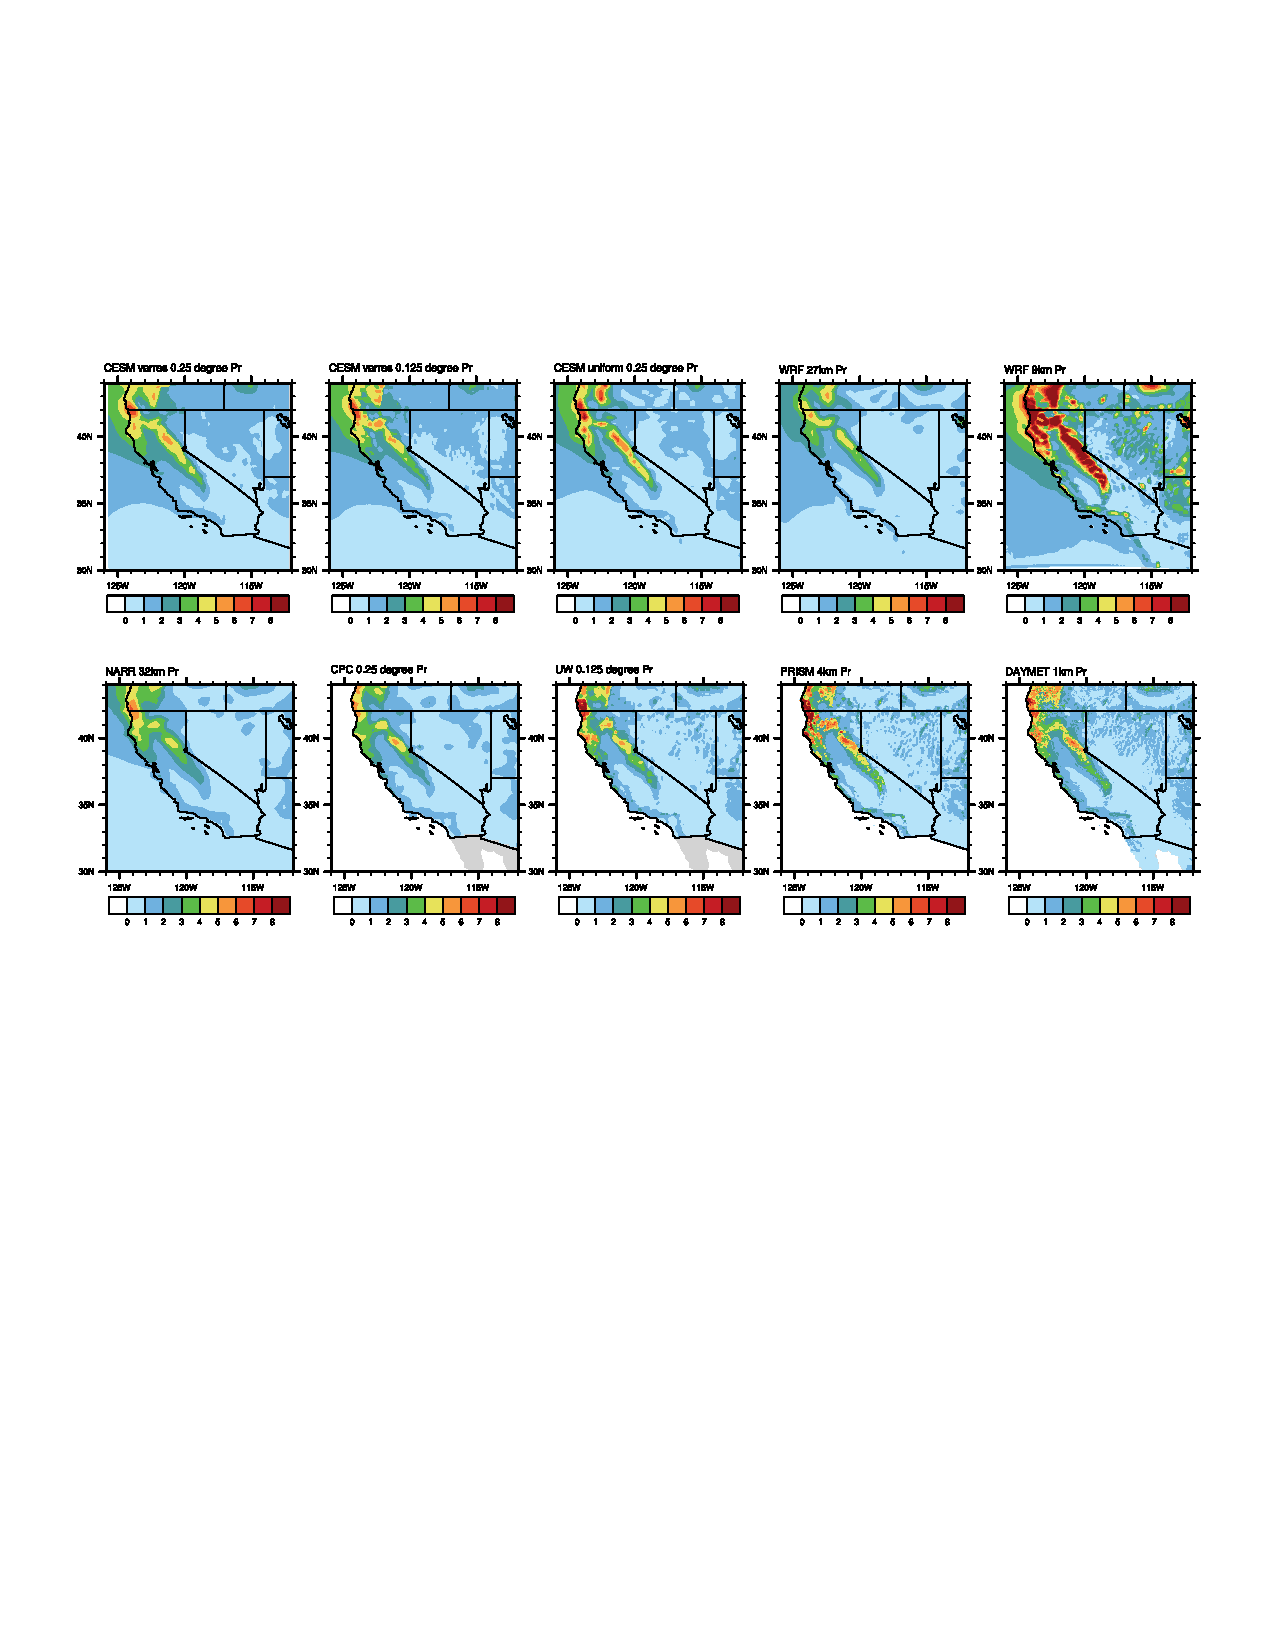
\includegraphics[width=6in]{pr.pdf}
\end{center}
\caption{Annual average daily total precipitation from models and reference datasets (mm/d). {\color{red} Change to four rows.  Use only one label bar.}} \label{fig:Figure12}
\end{figure}

\begin{figure}
\begin{center}
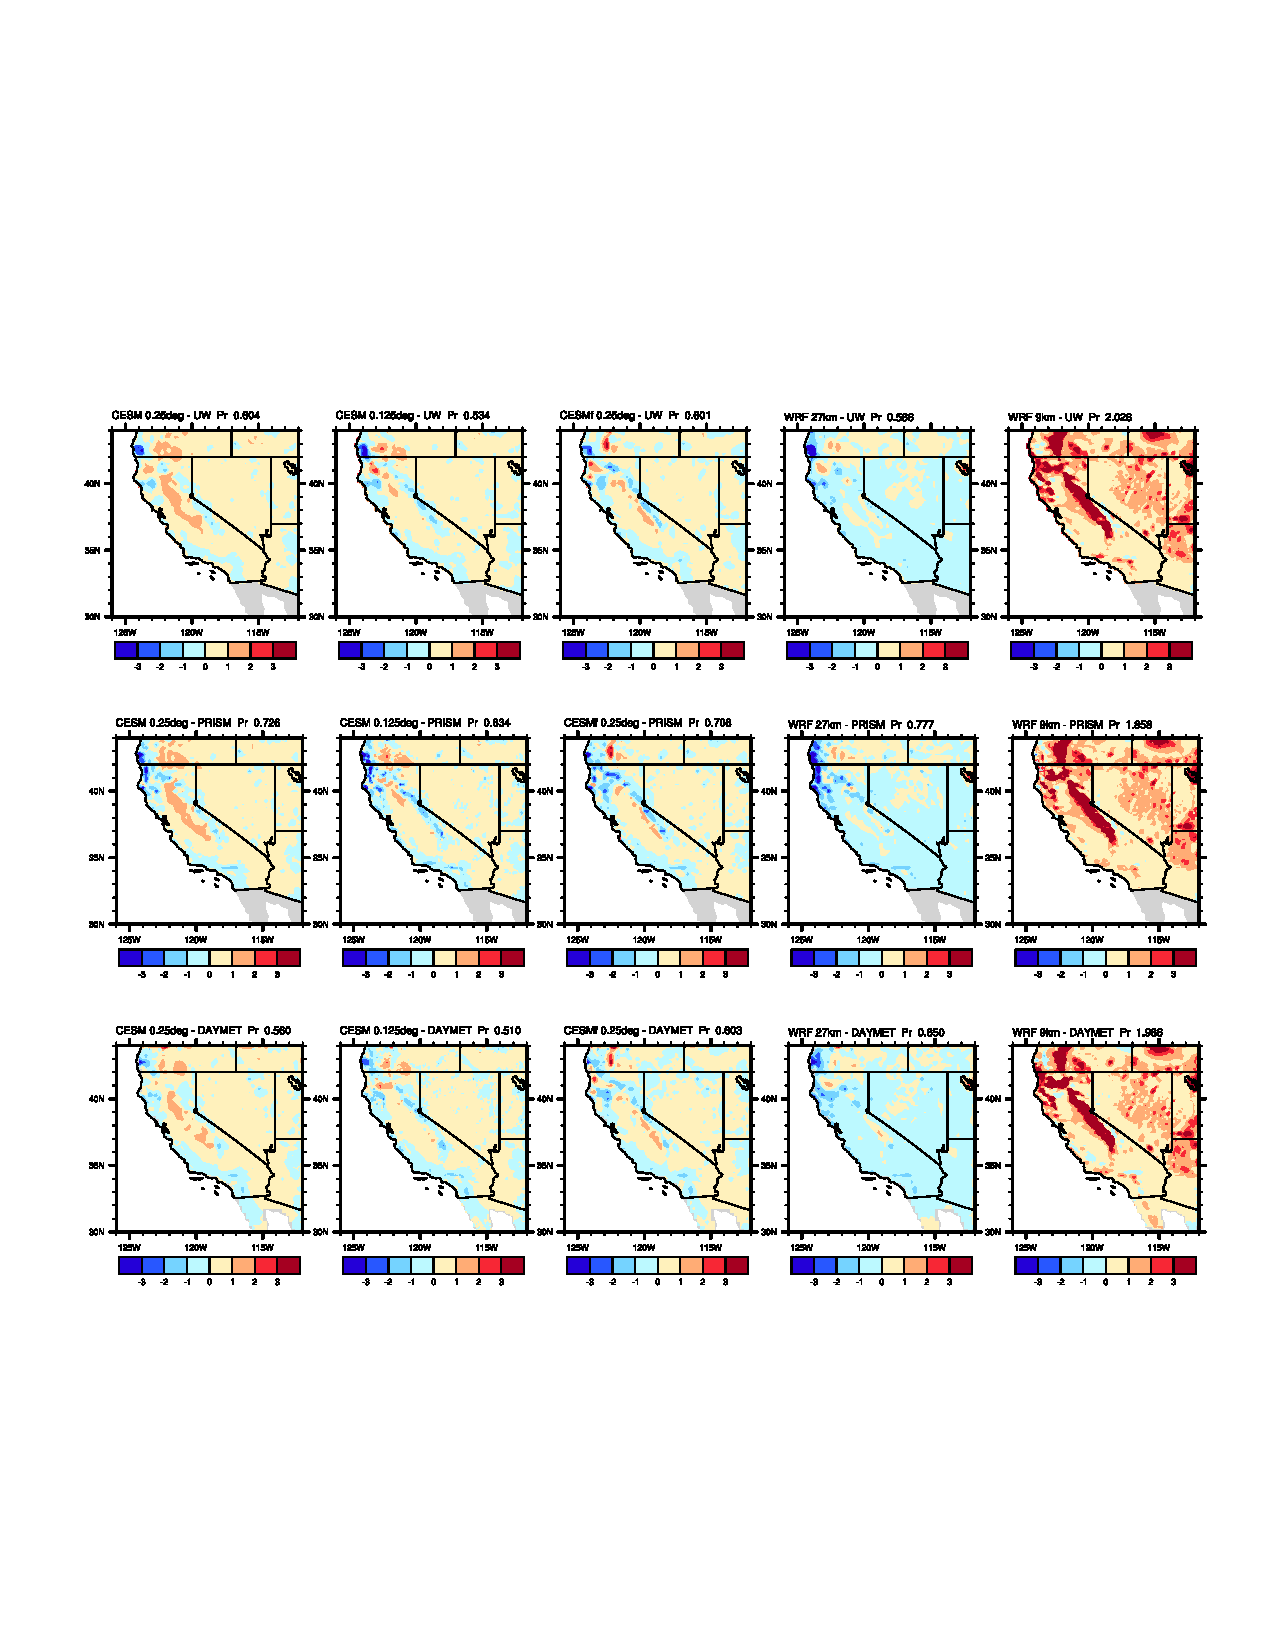
\includegraphics[width=6in]{pr_dif.pdf}
\end{center}
\caption{Difference between simulations and reference data for total precipitation (mm/d). {\color{red} Only use UW and PRISM.  Change to four rows.  Use only one label bar.}} \label{fig:Figure13}
\end{figure}

\begin{figure}
\begin{center}
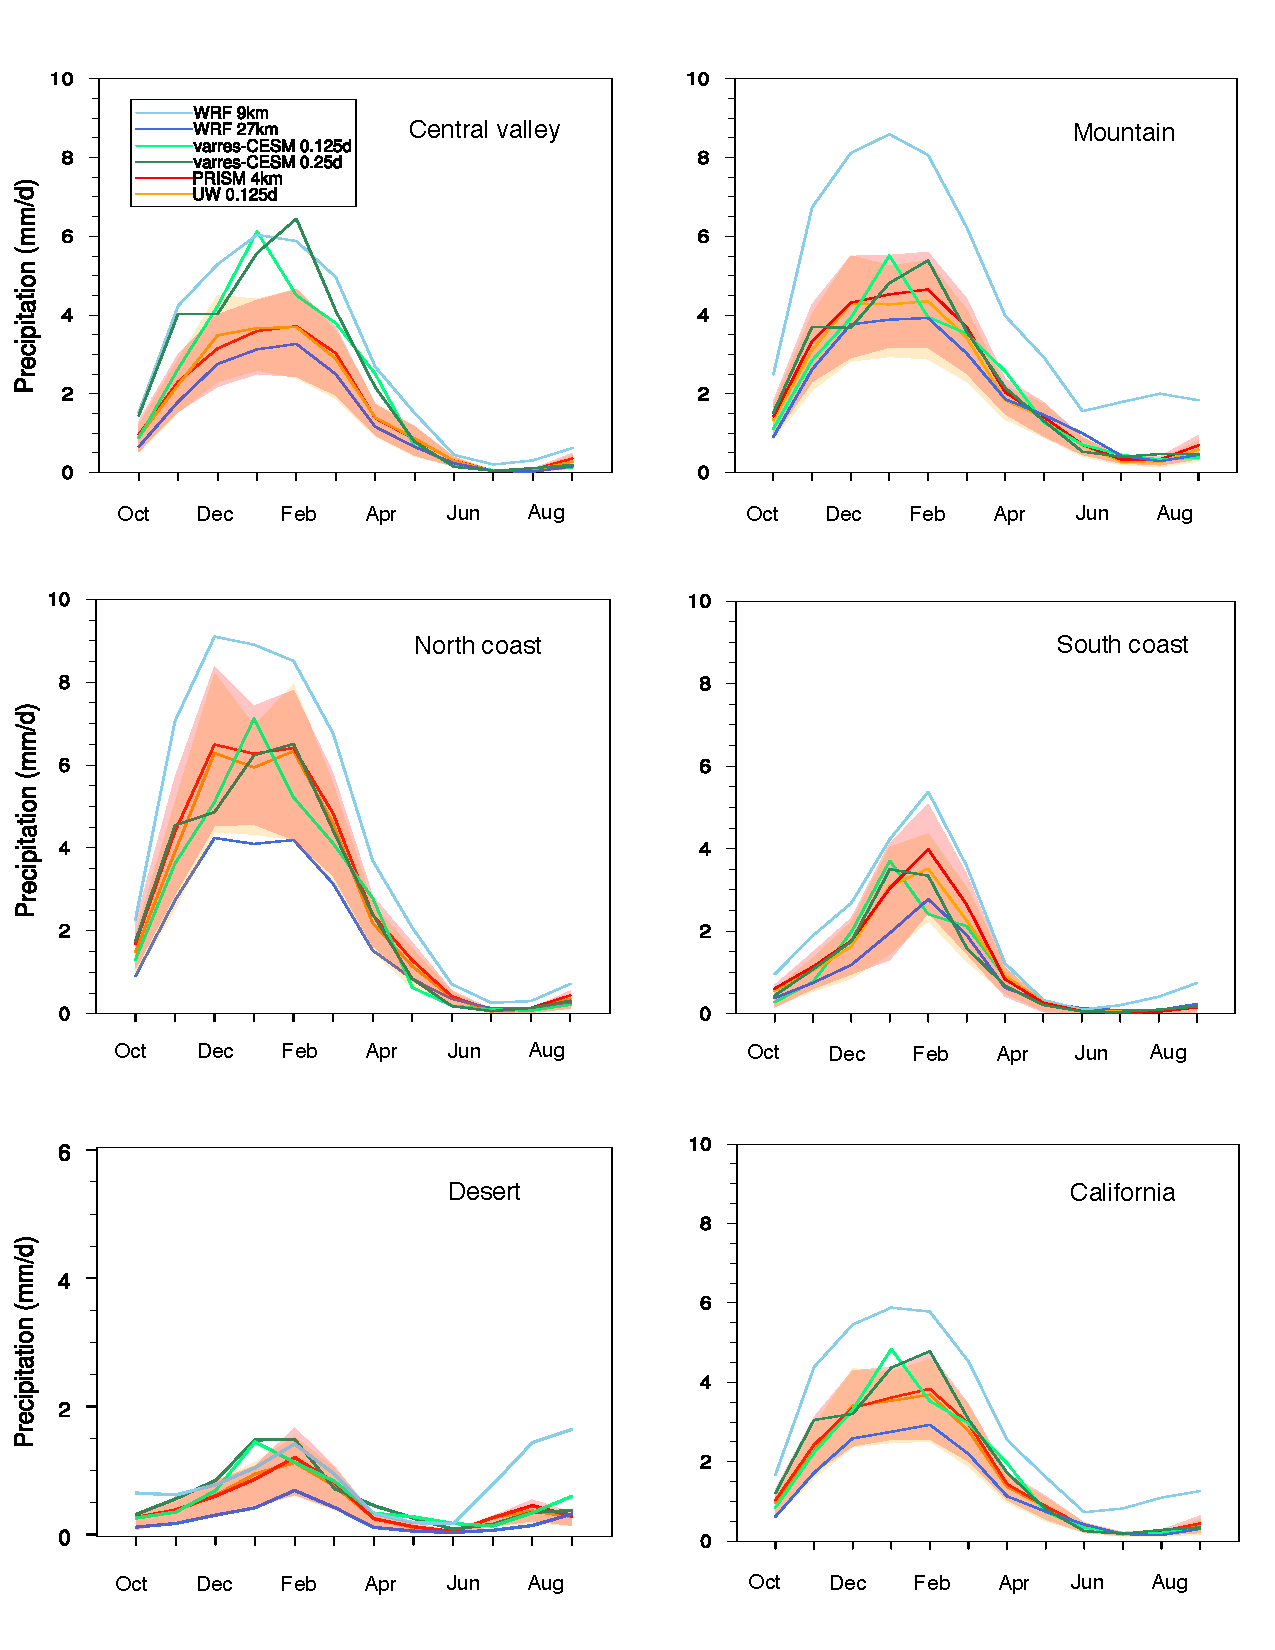
\includegraphics[width=6in]{trd_pr_allzones.pdf}
\end{center}
\caption{As Figure 8, but for monthly-average total precipitation (mm/d). {\color{red} Remove dots -- might need to put these on a separate plot.  Remove ``month'' from horizontal.  Change vertical label to Precipitation (mm/d).  Why do these plots start in September?  Change to January through December.}} \label{fig:Figure14}
\end{figure}

\begin{figure}
\begin{center}
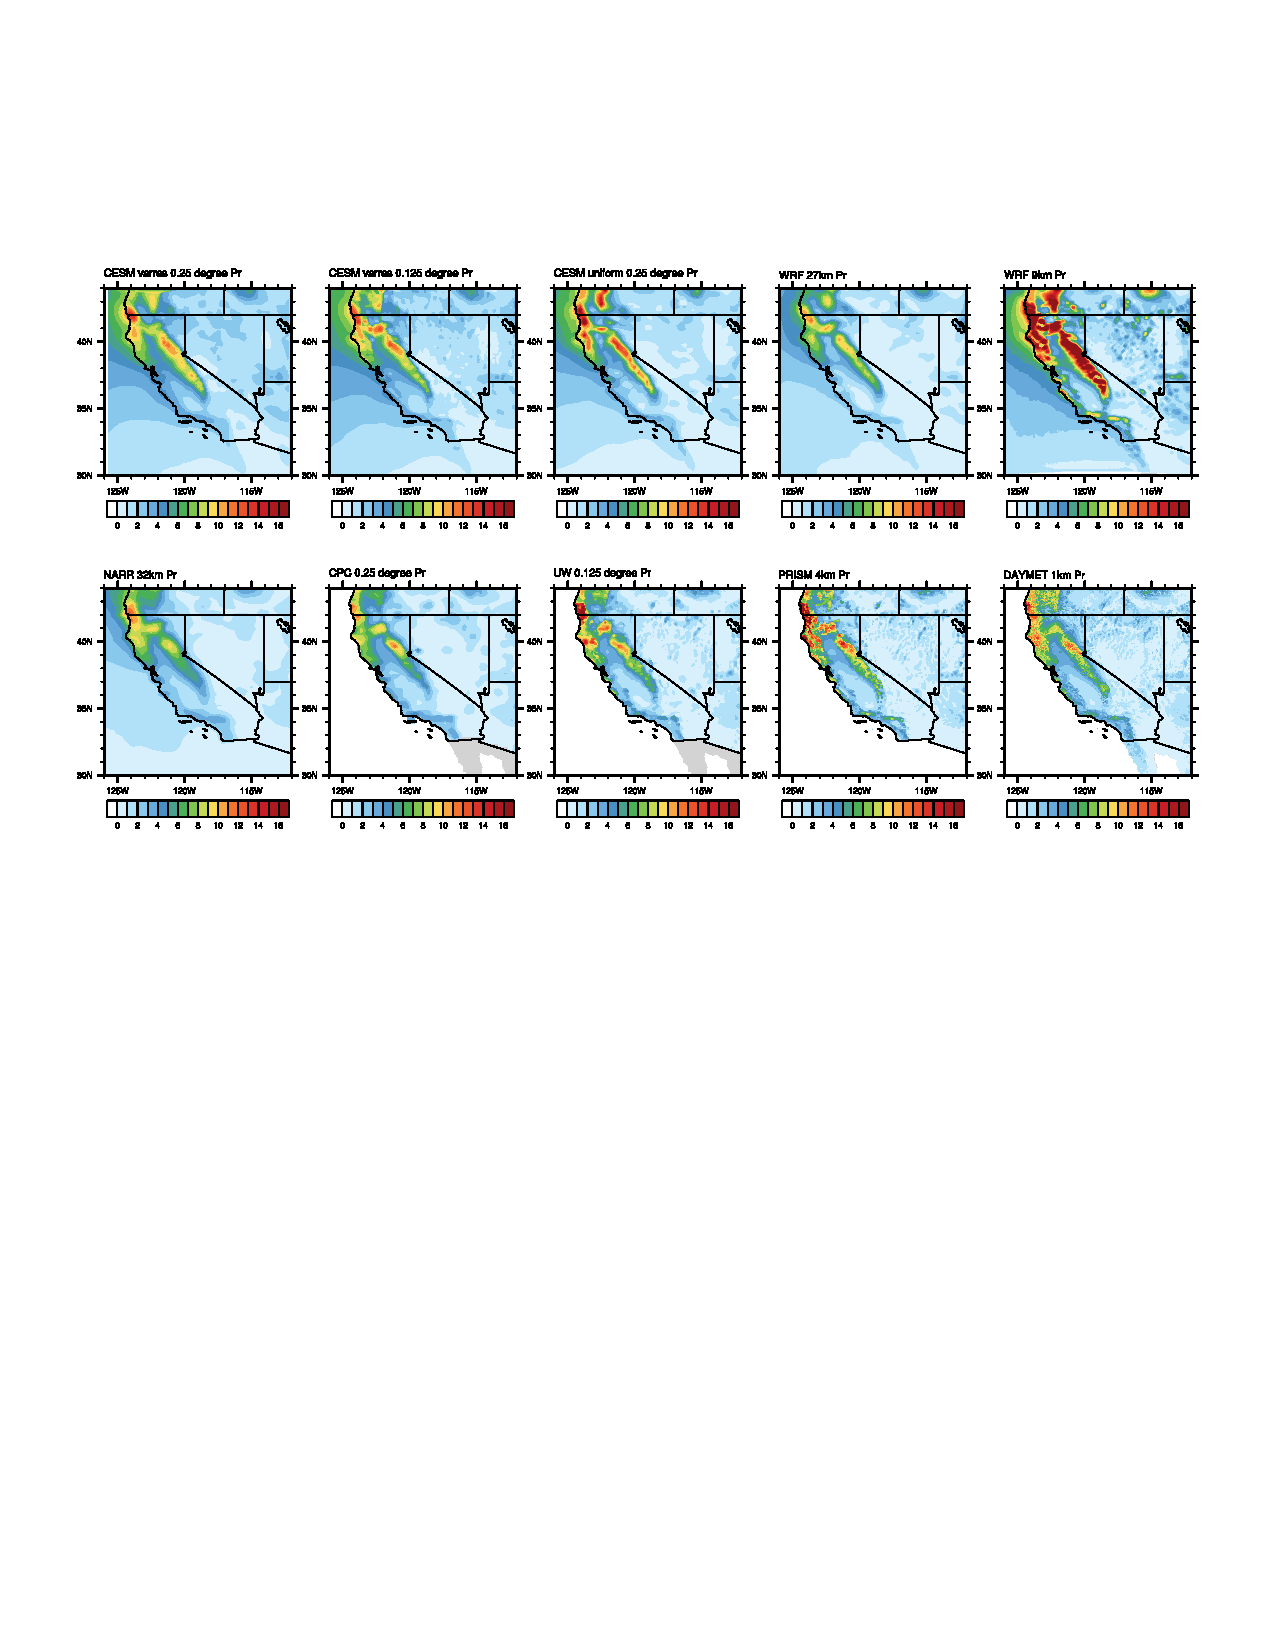
\includegraphics[width=6in]{pr_DJF.pdf}
\end{center}
\caption{As Figure 12, but for winter (DJF) total precipitation (mm/d). {\color{red} Change to four rows.  Use one label bar for all plots.}} \label{fig:Figure15}
\end{figure}

\begin{figure}
\begin{center}
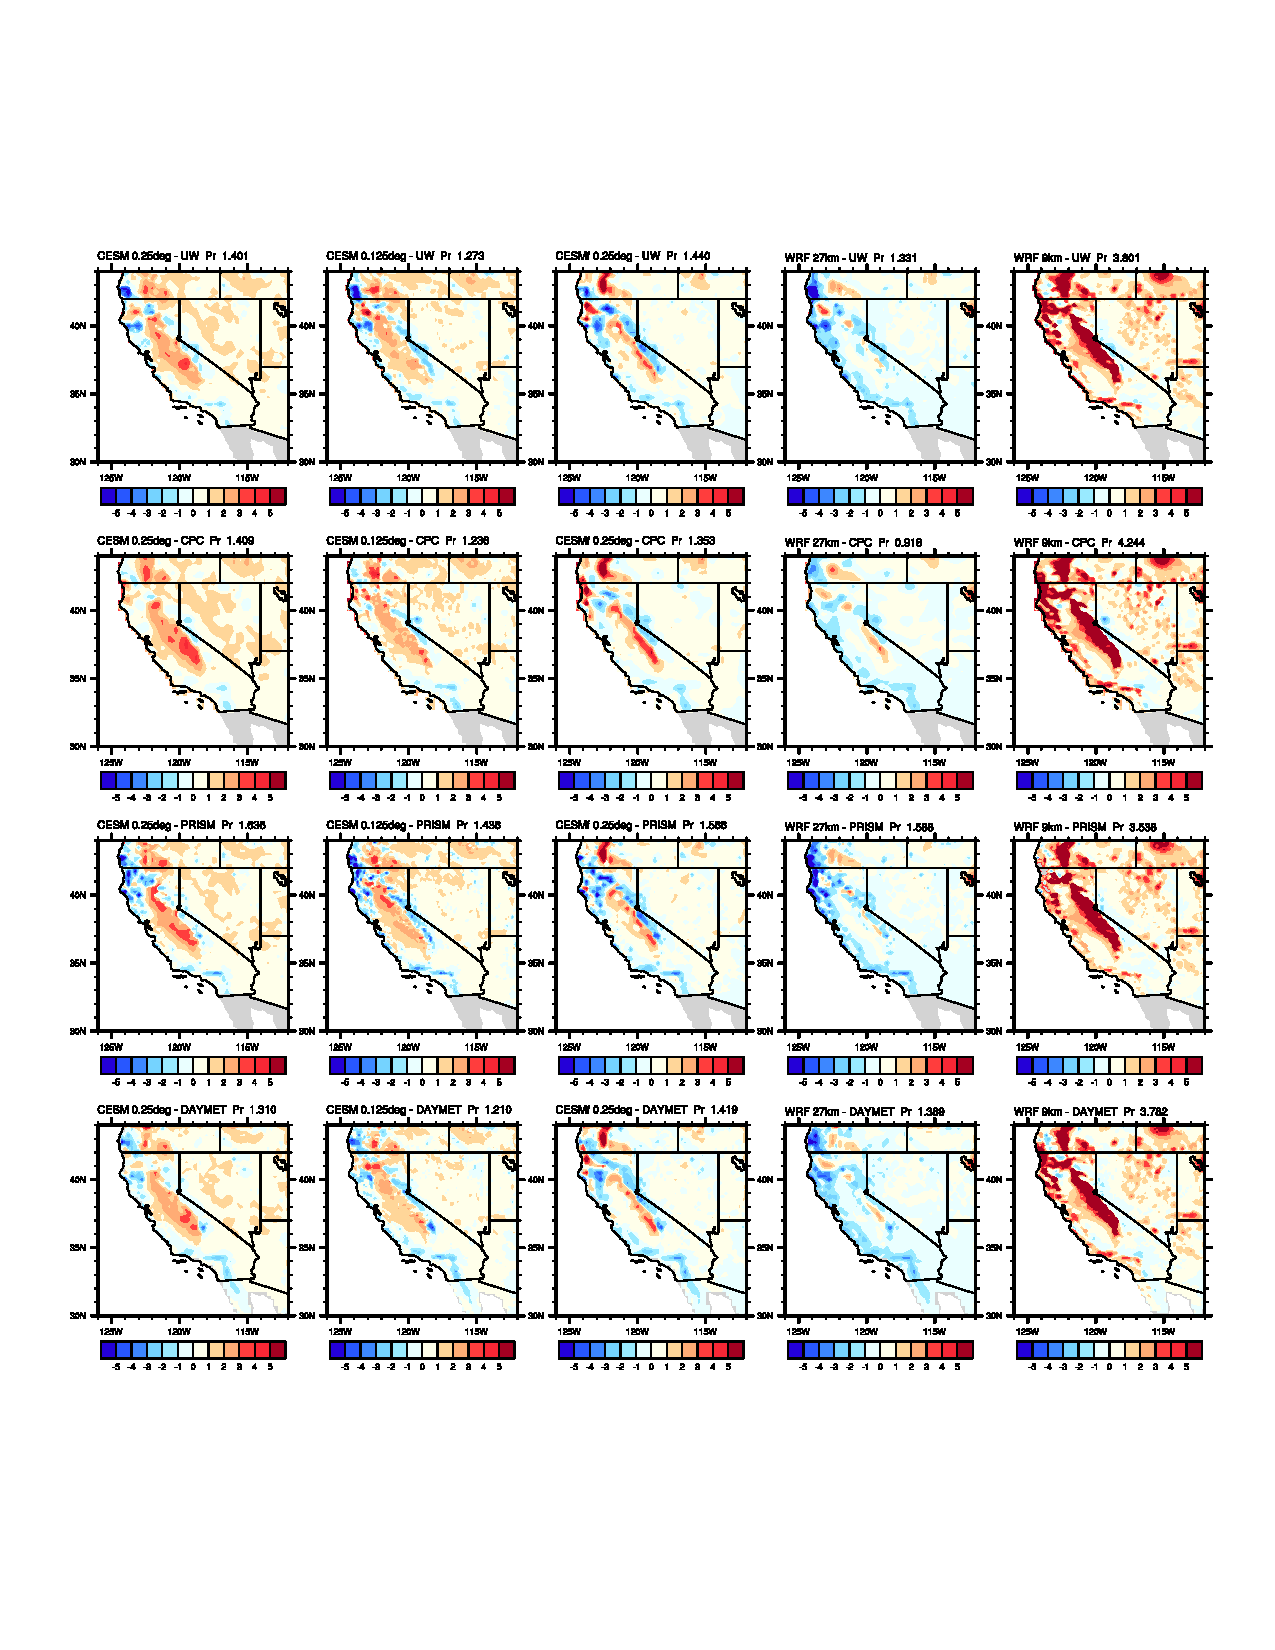
\includegraphics[width=6in]{pr_DJF_dif.pdf}
\end{center}
\caption{As Figure 13, but for winter (DJF) total precipitation (mm/d). {\color{red} Use only UW and PRISM.  Change to four rows.  Use only one label bar.}} \label{fig:Figure16}
\end{figure}

\begin{figure}
\begin{center}
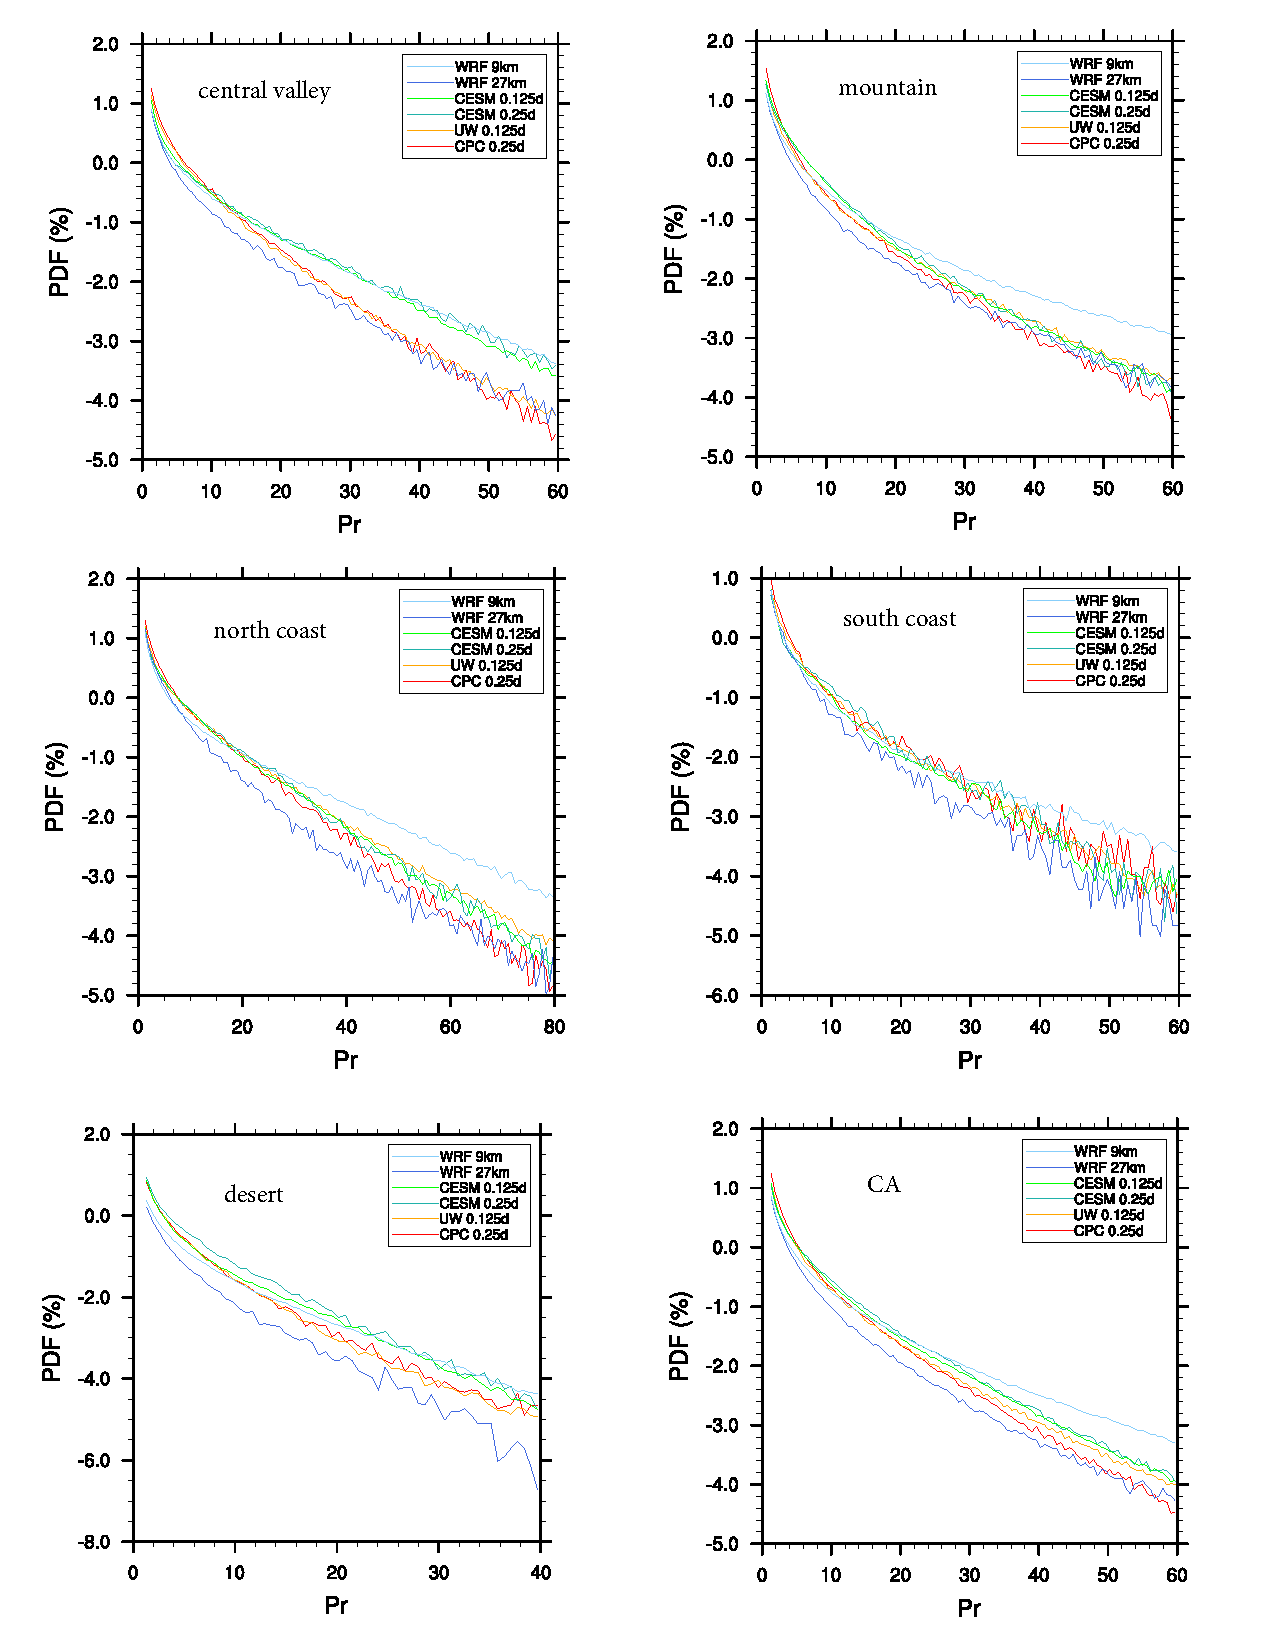
\includegraphics[width=6in]{PDF_pr_allzones_log_JJA.pdf}
\end{center}
\caption{Frequency distribution of winter Pr constructed from 26 years daily data (mm/d) (note that the vertical scale is logarithmic). {\color{red}Change vertical label to log$_{10}$ Frequency (\%).  Capitalize labels and change CA to California.  Only use one legend for all plots.  Use same horizontal range for all plots [0,80].  Use same vertical range for all plots [-5,2].}} \label{fig:Figure17}
\end{figure}

\begin{figure}
\begin{center}
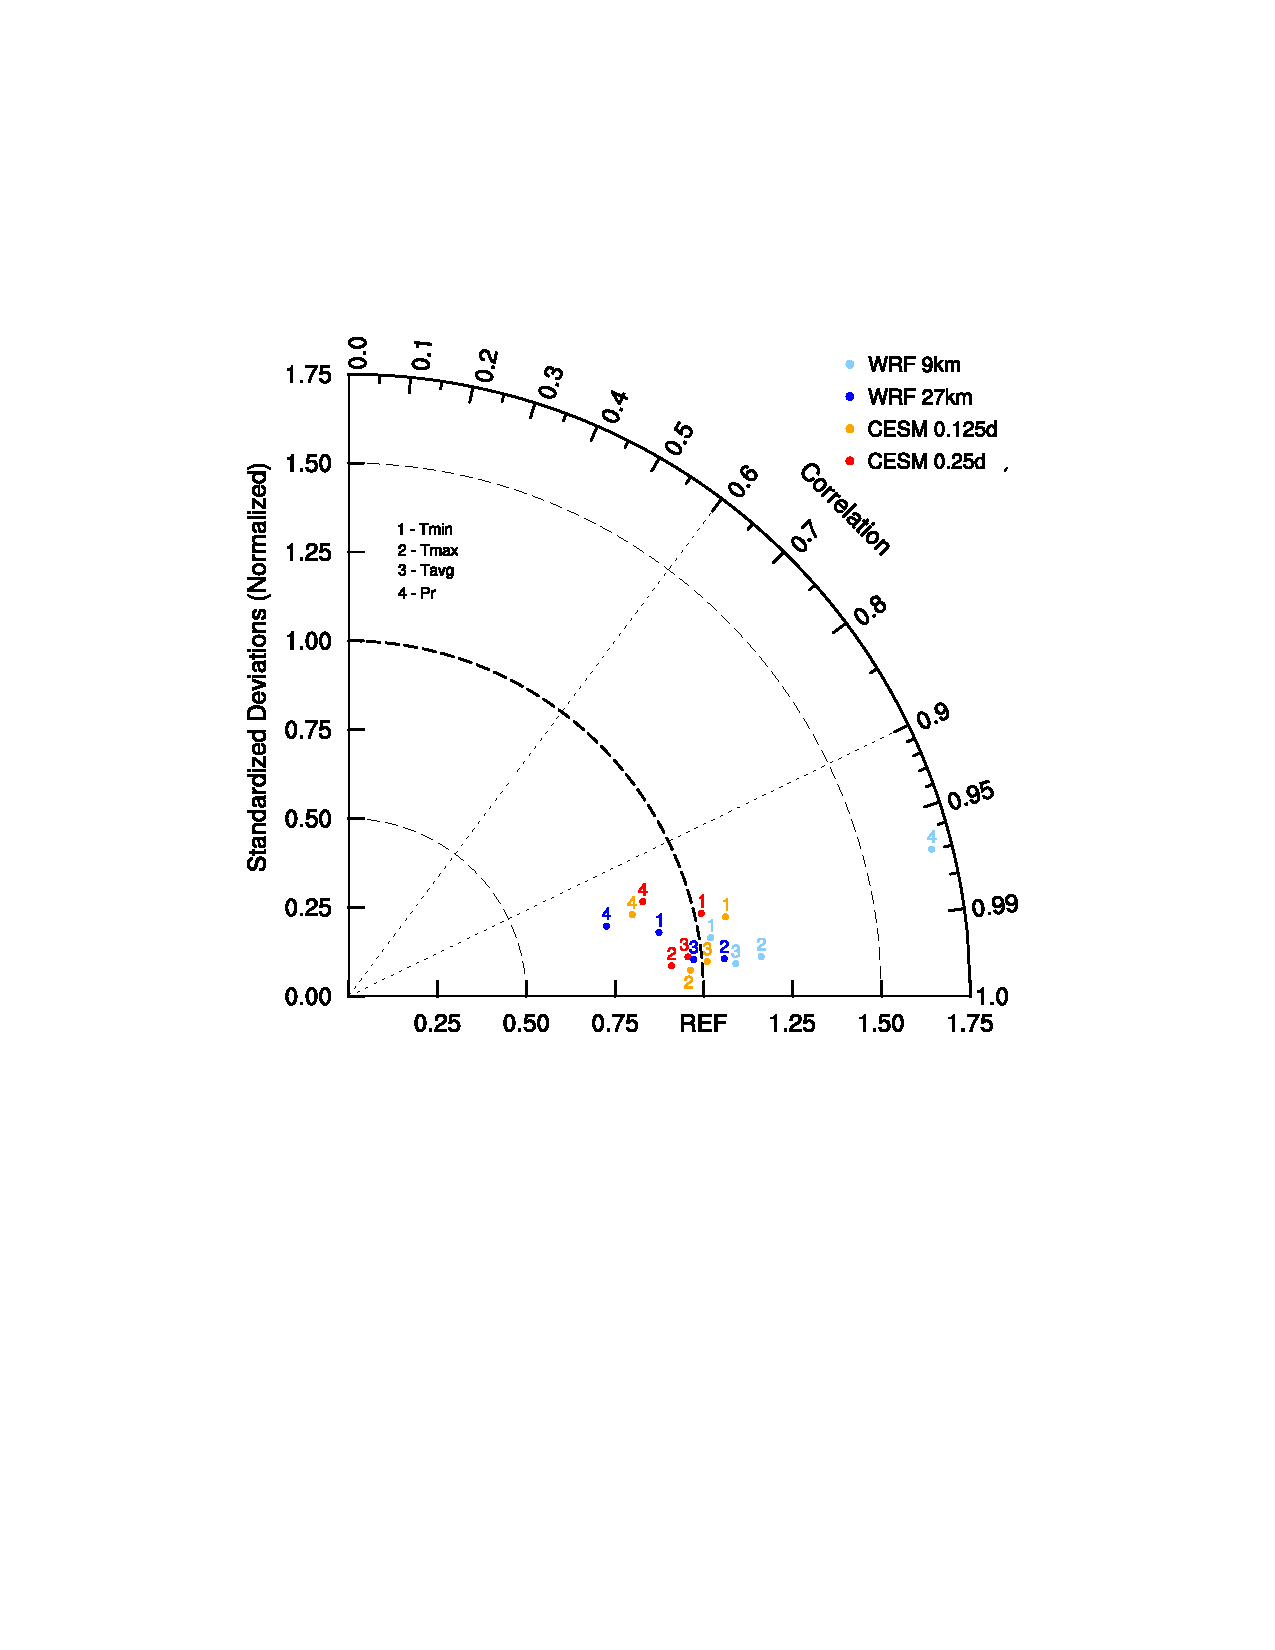
\includegraphics[width=6in]{taylor diagram.pdf}
\end{center}
\caption{Taylor diagram of annual climatology for the region of CA, using PRISM dataset as reference} \label{fig:Figure18}
\end{figure}

\section{Conclusions}

This work will motivate the use of varres-CESM for assessing climate change in CA over the coming century.

%Reference to Figure \ref{fig:Figure1}.

%%%%%%%%%%%%%%%%%%%%%%%%%%%%%%%%%%%%%%%%%%%%%%%%%%%%%%%%%%%%%%%%%%%%%
% ACKNOWLEDGMENTS
%%%%%%%%%%%%%%%%%%%%%%%%%%%%%%%%%%%%%%%%%%%%%%%%%%%%%%%%%%%%%%%%%%%%%
\acknowledgments

 \bibliographystyle{ametsoc2014}
 \bibliography{database2015}

%%%%%%%%%%%%%%%%%%%%%%%%%%%%%%%%%%%%%%%%%%%%%%%%%%%%%%%%%%%%%%%%%%%%%
% END OF AMSPAPER.TEX
%%%%%%%%%%%%%%%%%%%%%%%%%%%%%%%%%%%%%%%%%%%%%%%%%%%%%%%%%%%%%%%%%%%%%

\end{document}
